\documentclass[a4paper]{article}

\renewcommand{\textfraction}{0.05}
\renewcommand{\topfraction}{0.85}
\renewcommand{\bottomfraction}{0.85}
\renewcommand{\floatpagefraction}{0.90}

\usepackage{graphicx}
\usepackage{url}
\usepackage{subcaption}
\usepackage{pdfpages}
\usepackage{booktabs}
\usepackage[section]{placeins}

\usepackage{color}
\definecolor{rltbrightred}{rgb}{1,0,0}
\definecolor{rltred}{rgb}{0.75,0,0}
\definecolor{rltdarkred}{rgb}{0.5,0,0}
%
\definecolor{rltbrightgreen}{rgb}{0,0.75,0}
\definecolor{rltgreen}{rgb}{0,0.5,0}
\definecolor{rltdarkgreen}{rgb}{0,0,0.25}
%
\definecolor{rltbrightblue}{rgb}{0,0,1}
\definecolor{rltblue}{rgb}{0,0,0.75}
\definecolor{rltdarkblue}{rgb}{0,0,0.5}
%
\definecolor{webred}{rgb}{0.5,.25,0}
\definecolor{webblue}{rgb}{0,0,0.75}
\definecolor{webgreen}{rgb}{0,0.5,0}

\usepackage[pdftex,
        colorlinks=true,
        urlcolor=rltblue,               % \href{...}{...}
        anchorcolor=rltbrightblue,
        filecolor=rltgreen,             % \href*{...}
        linkcolor=rltred,               % \ref{...} and \pageref{...}
        menucolor=webblue,
        citecolor=webgreen,
        pdftitle={MTF Mapper documentation},
        pdfauthor={F. van den Bergh},
        pdfsubject={MTF Mapper documentation},
        pdfkeywords={MTF MTF50 acuity sharpness slanted edge autofocus},
        pdfpagemode=UseNone,
        bookmarksopen=true]{hyperref}


\addtolength{\textwidth}{2cm}
\addtolength{\hoffset}{-1cm}
\addtolength{\textheight}{2cm}
\addtolength{\voffset}{-1cm}
\setlength{\parindent}{0pt}
\setlength{\parskip}{1ex}

\title{MTF Mapper user guide}
\author{Frans van den Bergh (fvdbergh\#at\#gmail\#dot\#com)}

\begin{document}
\maketitle

\tableofcontents

\newpage

\section{What can I do with MTF Mapper?}
\label{sec:overview}
The MTF mapper package offers a collection of tools to measure Modulation
Transfer Function (MTF) values across edges in images. One popular metric
derived from the MTF is called MTF50, which corresponds to perceived 
sharpness of edges; this means that the MTF mapper tools can be used to 
evaluate camera lens sharpness, as well as autofocus behaviour.

MTF Mapper comes with a variety of test charts which can be printed by an
end user.  Some of the output types that it supports requires such MTF
Mapper test charts, but for other output types any suitable test chart can
be used, including one of your own design.  An important design goal of MTF
Mapper was to automate the process as far as possible, meaning you no longer
have to manually draw rubberband boxes around edges.

Here are some of the things you can do with MTF Mapper:
\begin{itemize}
\item
Check whether your lens is performing as expected, e.g., whether one side of
the lens is perhaps unacceptably soft;
\item
Check whether your lens is front-focusing or back-focusing;
\item
Optimize your camera's auto-focus micro-adjust (or fine-tuning), or if you
have a Sigma Art lens, MTF Mapper can help you to calibrate focus using the
dock;
\item 
Measure how much (if any) focus shift your lens experiences on stopping
down;
\item
Measure longitudinal chromatic aberration;
\item
Measure and visualize camera system MTF / SFR curves.
\end{itemize}

To get a more visual idea of what you can do with MTF Mapper, consider the
following types of output you can produce with it:
\subsection{Annotated images}
\label{sec:annotated_images}
In an annotated output image, the MTF50 value of an edge is printed on top
of the edge itself. These annotated images are useful to evaluate the sharpness
of your camera across the entire image, but you want to see the numbers
(right part of Figure~\ref{fig:annotated_example}), rather than a plot.

\begin{figure}[!ht]
\centering
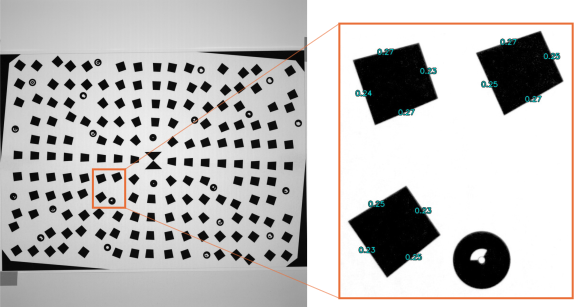
\includegraphics[width=0.85\textwidth]{figures/annotation_example}
\caption{Left: A sample image of a printed MTF Mapper ``lensgrid'' chart.
Right: A close-up crop of the output produced by MTF Mapper. The Cyan
numbers indicate the MTF50 value of each edge in cycles per pixel.}
\label{fig:annotated_example}
\end{figure}

\begin{figure}[!ht]
\centering
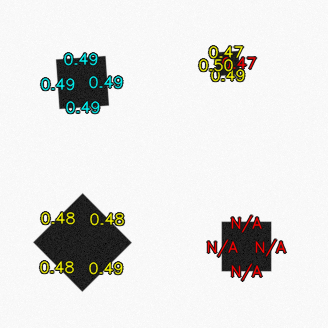
\includegraphics[width=0.45\textwidth]{figures/annotation_colours}
\caption{Examples of some of the conditions that affect the colour of the
annotation text. Ideally, all your annotations should be Cyan.}
\label{fig:annotated_colours}
\end{figure}

The colour of the annotation text is Cyan if MTF Mapper thinks everything is
fine, but will change to Yellow (edge orientation is close to $45^\circ$, or the edge is
shorter than about 25 pixels, which may result in inaccurate results) and
finally Red (better not to trust these, rather fix the problem). The text
may also read ``N/A'', which usually means the edge was either at an
orientation of $0^\circ$ or at $90^\circ$. (see
Figure~\ref{fig:annotated_colours})

\newpage

\subsection{MTF surface images}
Derived from the same input images as used to produce \textsf{Annotated
images}, the MTF50 surface images are a colour representation of your MTF50
values measured across your camera's sensor.

\begin{figure}[!ht]
\centering
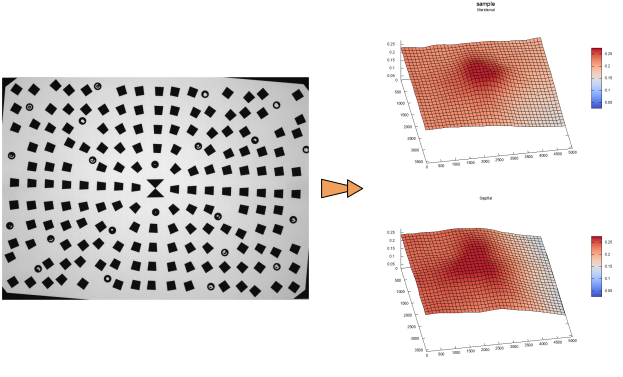
\includegraphics[width=0.85\textwidth]{figures/surface_example}
\caption{Left: A sample image of a printed MTF Mapper ``lensgrid'' chart.
Right: MTF Mapper's ``grid'' output, which is a 3D plot of MTF50 values (as
the height) across the image.
}
\label{fig:surface_example}
\end{figure}

\begin{figure}
\centering
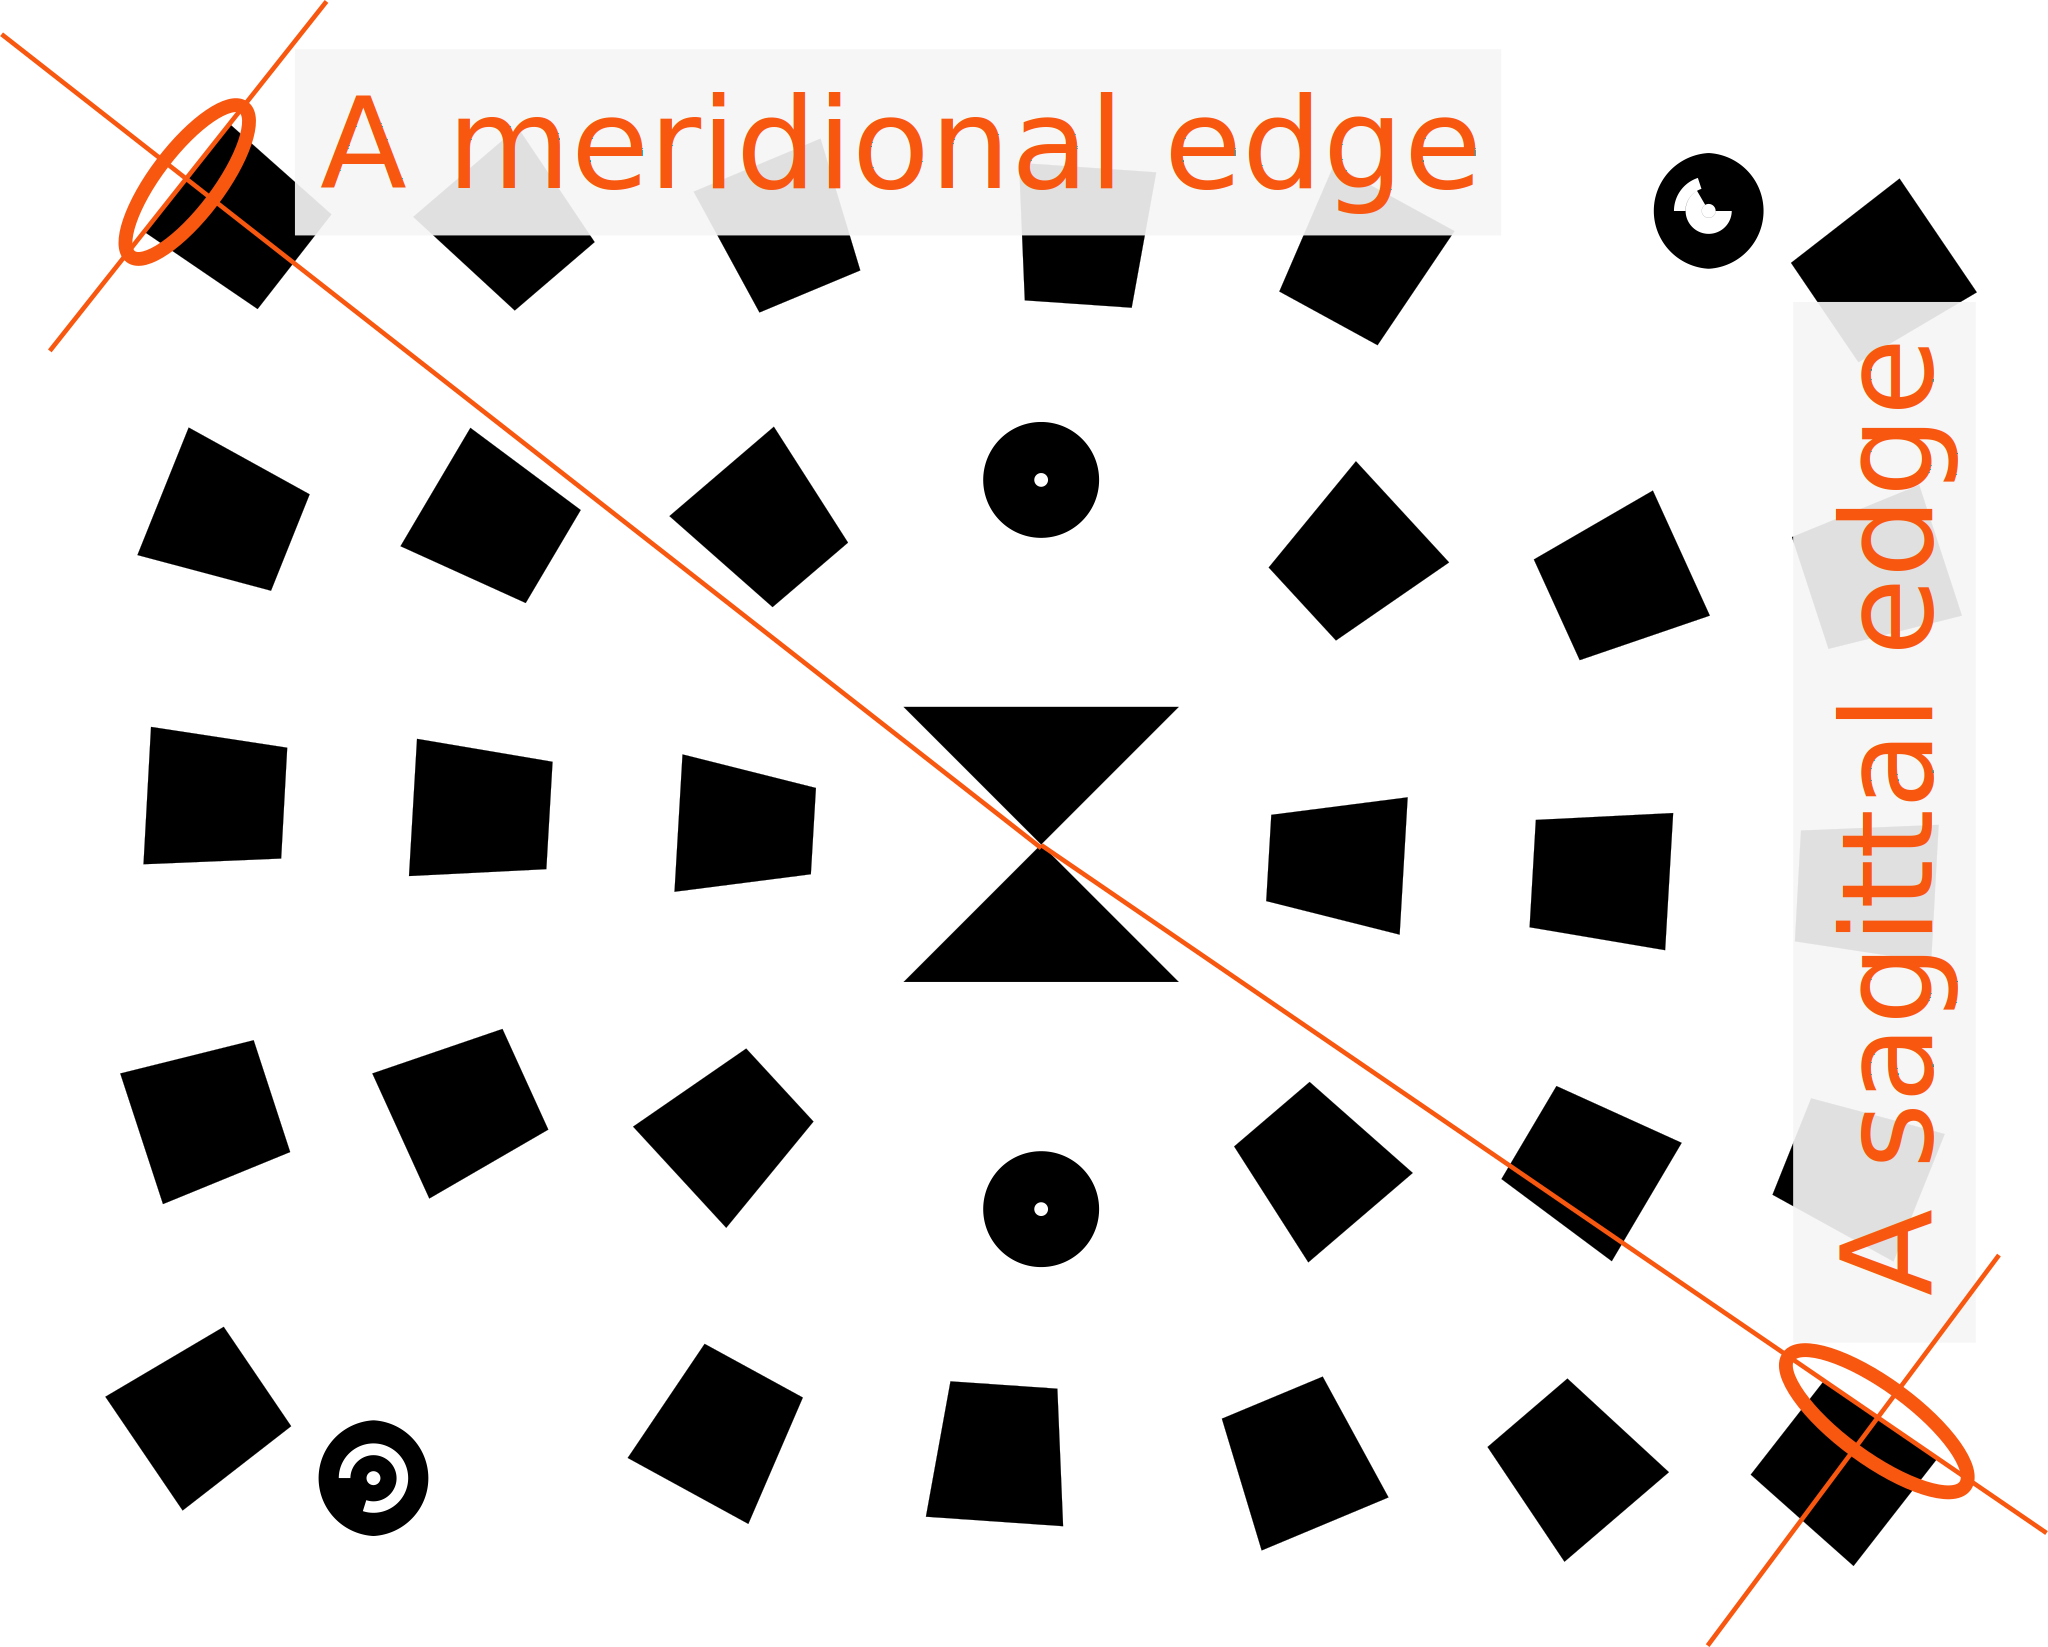
\includegraphics[width=0.35\textwidth]{figures/meridional_sagittal}
\caption{Meridional vs Sagittal directions.}
\label{fig:ms_directions}
\end{figure}

Note that MTF Mapper's output is split into \emph{meridional} and
\emph{sagittal} plots; the main reason for this is that most cameras have
distinctly different performance along the meridional and sagittal
directions. The sagittal MTF50 values are derived from edges that are
oriented along radial lines (with respect to the centre of the image), and
the meridional MTF50 values come from the other edges, that are oriented to
be tangential to a circle centred at on the image; see
Figure~\ref{fig:ms_directions}.

\subsection{Lens profile MTF plots} 
\label{sec:lens_profile}
MTF Mapper can produce plots that are similar to those produced by lens
manufacturers, which show contrast plotted as a function of distance from
the lens centre, at a few selected spatial resolution choices.

\begin{figure}[!ht]
\centering
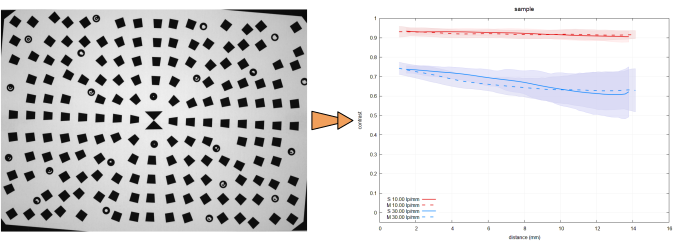
\includegraphics[width=0.85\textwidth]{figures/lensprofile_example}
\caption{Left: A sample image of a printed MTF Mapper ``lensgrid'' chart.
Right: A lens MTF profile, showing contrast at 10 lp/mm and 30 lp/mm as a
function of distance from the centre of the lens, for both the meridional
and sagittal directions.}
\label{fig:lensprofile}
\end{figure}

Note that MTF Mapper's lens profile plots cannot exactly reproduce the MTF
plots published by the lens manufacturer, mostly because MTF Mapper measures
\emph{system} MTF, which is a combination of lens MTF and the camera
sensor's MTF.  Also note that some manufacturers publish theoretical rather
than measured MTF.  Having said that, the shape of MTF Mapper's lens profile
plots should be similar to the manufacturer's plot, but the absolute
contrast value will be somewhat lower.

\subsection{Profile data sets / Autofocus fine-tuning} 
This particular MTF Mapper output is specifically designed to work with a
$45^\circ$ test chart, like MTF Mapper's ``perspective'' chart type. The
details on using this method to adjust DSLR autoforcus fine-tuning are
discussed in Section~\ref{sec:autofocus}.

\begin{figure}[!ht]
\centering
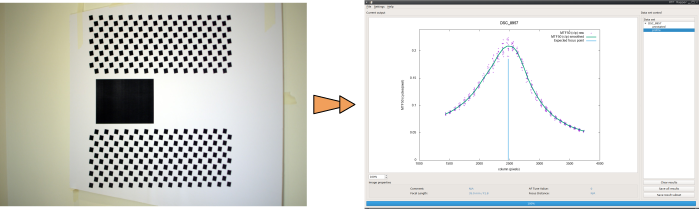
\includegraphics[width=0.85\textwidth]{figures/profile_example}
\caption{Left: A sample image of a printed MTF Mapper ``perspective'' chart.
Right: MTF50 values plotted as a function of distance.}
\label{fig:profile_example}
\end{figure}

The vertical blue line in Figure~\ref{fig:profile_example} shows the
location of the edge used for AF, and the green curve shows the sharpness in
relation to this edge, i.e., we can infer from this plot that the camera AF
has been successfully adjusted in this example.

\newpage

\subsection{Plots of SFR curves (or MTF curves)}
\label{sec:sfr_curve}
Derived from the same input images as used to produce \textsf{Annotated
images}, MTF Mapper can plot the SFR curve (or the MTF curve, if you prefer)
of a given edge by interactively selecting the edge within the GUI by
clicking on the Cyan text annotation. By holding shift while left-clicking
on the edge, up to three different edges can be selected and plotted
together; you can even select all three images from different
\textsf{Annotated image} outputs to compare, say, the same test chart edge
across different aperture settings of the lens.

\begin{figure}[!hb]
\centering
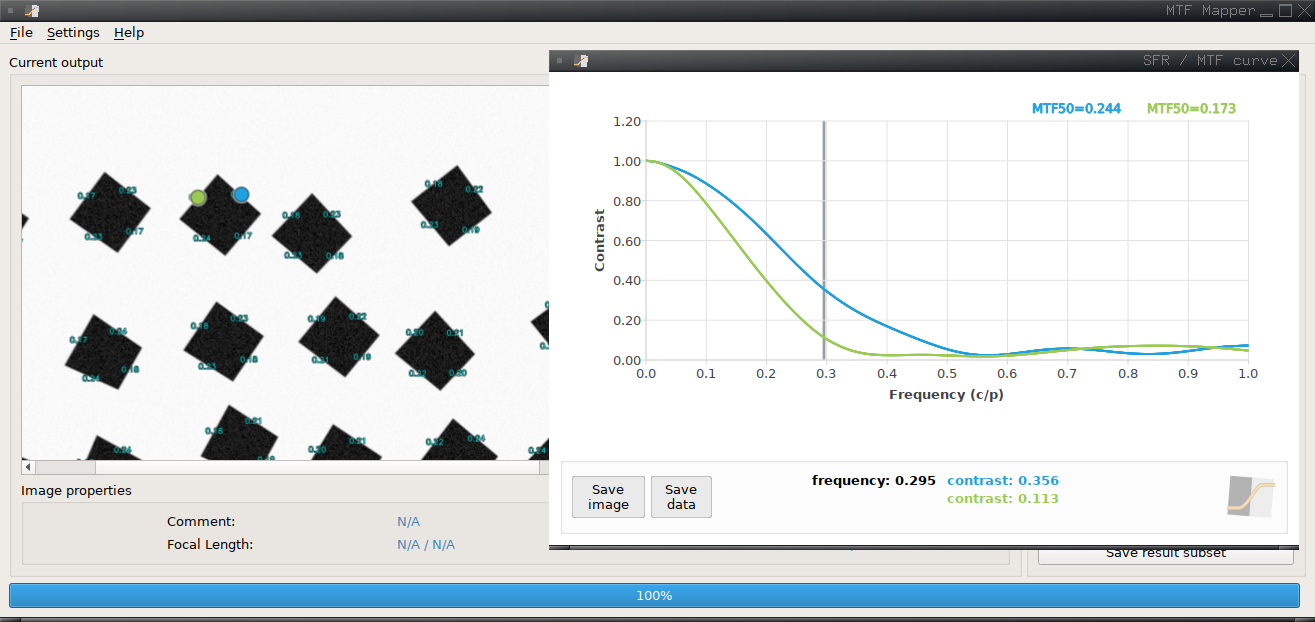
\includegraphics[width=0.85\textwidth]{figures/sfr_example}
\caption{Two edges have been selected. One is slightly out of focus, the other sharper,
The pop-up window displays the SFR curves for both of these
edges by plotting contrast vs frequency.}
\label{fig:sfr_example}
\end{figure}

Note that even though the example presented in Figure~\ref{fig:sfr_example}
relied on the GUI to perform the edge selection, the actual SFR data of any 
edge can readily be extracted using the command line version of MTF Mapper 
for batch processing.

\newpage

\subsection{Checking test chart orientation}
\label{sec:chart_orientation}
Most of the MTF Mapper outputs rely on setting up the chart to be
perpendicular to the optical axis of the lens, or put differently, you want
your camera's sensor to be parallel to the test chart. If your test chart is not
perfectly parallel to the sensor, it might appear that, say, the right side of
your lens appears soft (e.g., it would look a little like the MTF surface
shown in Figure~\ref{fig:surface_example}). You can only really say that the
right side of the lens is in fact soft if you have confirmed that your
set-up is good.

There are many different methods of aligning your test chart; the simplest
method is to hold a small mirror flat against the centre of the test chart: if your camera
can see itself looking back, you are close. Another approach is to use the
built-in ``chart orientation'' option provided by MTF Mapper. This
absolutely requires a ``lensgrid'' style test chart, since MTF Mapper looks
at the circular fiducial patterns to measure the chart orientation.
Figure~\ref{fig:chart_orientation_example} shows the output: you ultimately
want to bring the \emph{yaw} and \emph{pitch} angles down to below
$1^\circ$, the lower the better. We can clearly see that the yaw angle is
about $2.68^\circ$ to the right, so in this case it is more likely that the
lens is fine (no tilted elements), but rather that the set-up has to be
adjusted slightly.

\begin{figure}[!ht]
\centering
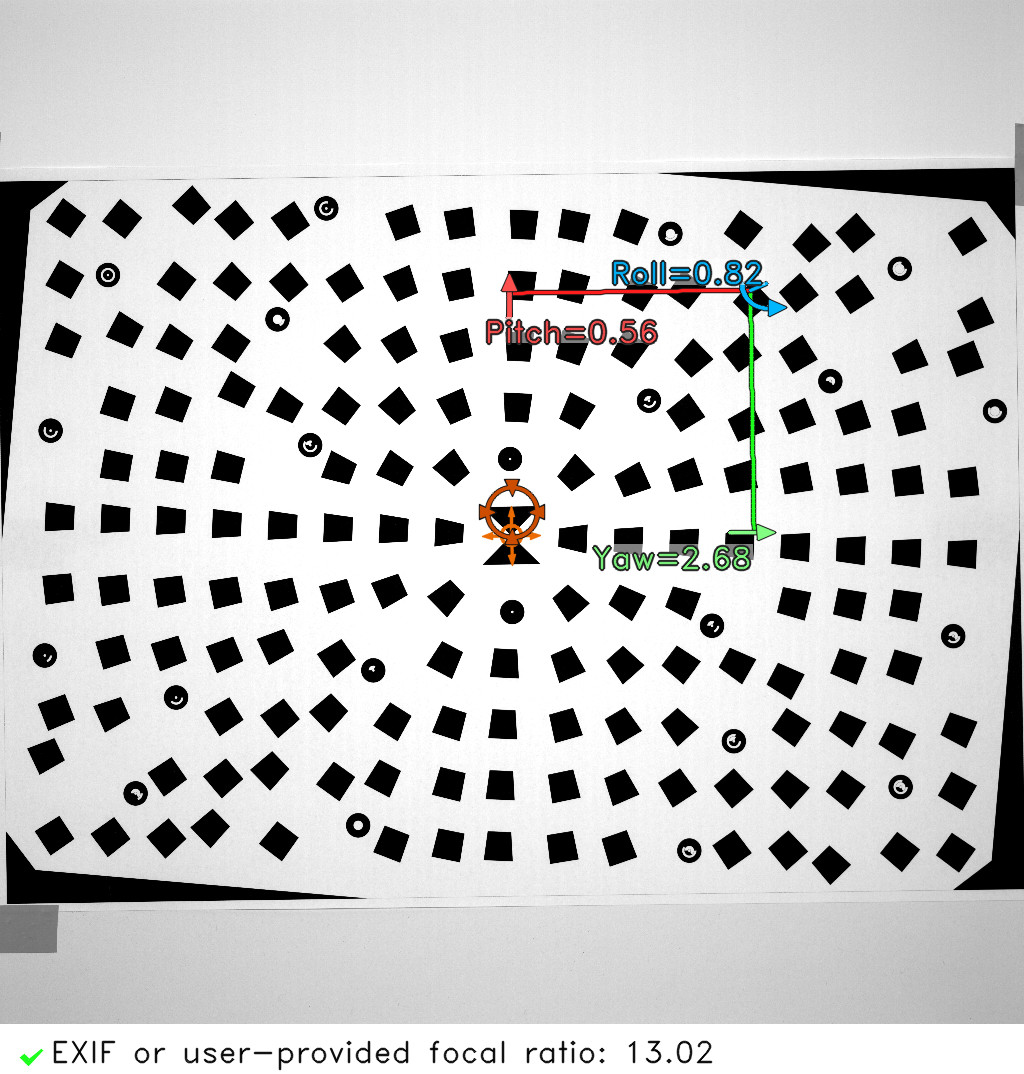
\includegraphics[width=0.75\textwidth]{figures/orientation_example}
\caption{Sample chart orientation output. As indicated by the $2.68^\circ$
yaw angle, this chart is tilted so that the right side of the chart is sligthly further
from the camera compared to the left side.}
\label{fig:chart_orientation_example}
\end{figure}

\newpage

\subsection{Measure the exact focus position (per colour subset if you want)}
\label{sec:focus_distance}
MTF Mapper can also measure the exact focus position of your camera. If this
sounds odd to you, you might be onto something. Normally one would expect focus
position to be handled either by the autofocus mechanism, or by the
photographer. However, if you have a manual focus lens and you want to
adjust the focus distance to an exact value, perhaps in some machine vision
application, then MTF Mapper can help. 

\begin{figure}[!ht]
\centering
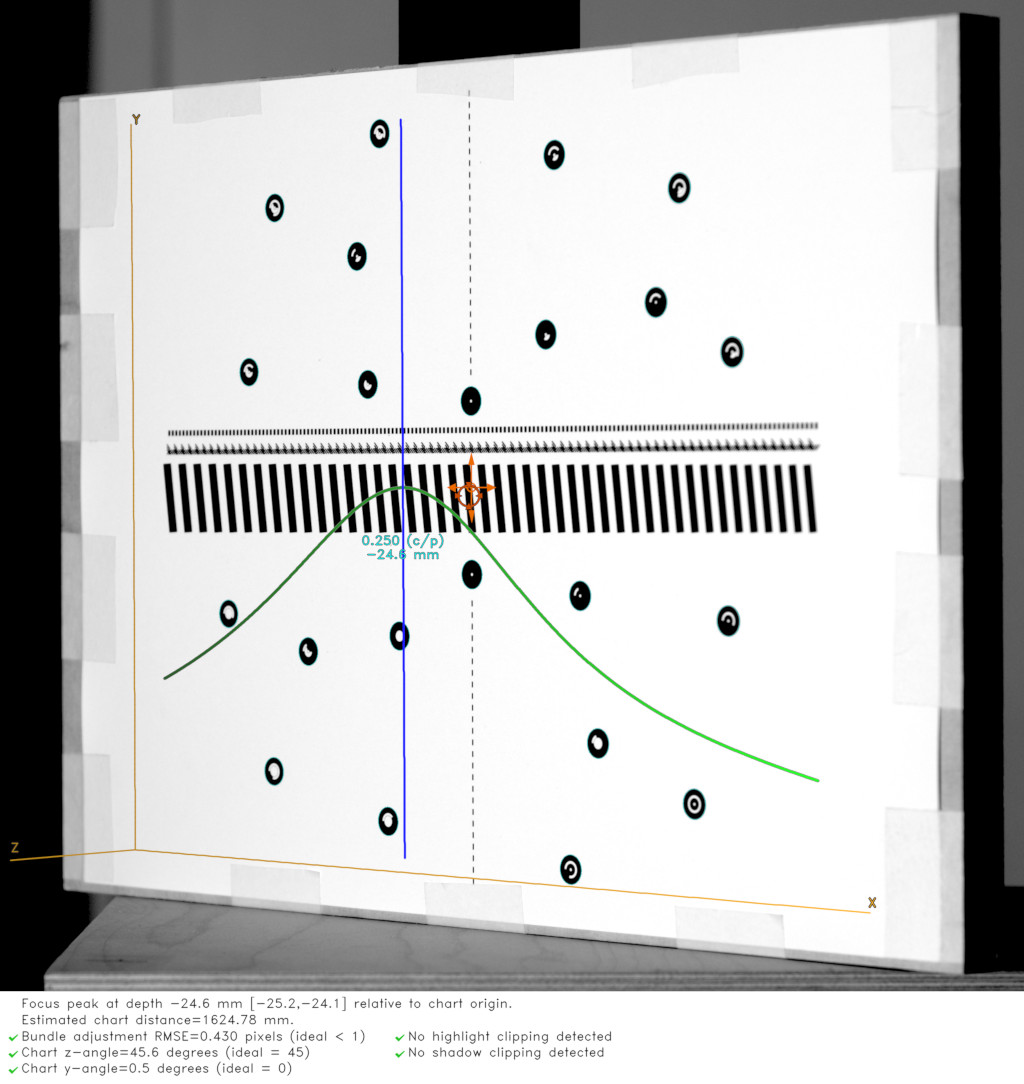
\includegraphics[width=0.85\textwidth]{figures/focus_peak_example}
\caption{From the ``focus'' type MTF Mapper chart, mounted at a $45^\circ$
degree angle, MTF Mapper can directly measure the depth-of-field curve
(which was drawn back onto the test chart image in green),
which also gives you the distance of best focus (blue line).}
\label{fig:focus_example}
\end{figure}

MTF Mapper can be used to measure focus shift in object space, measuring the
exact shift in millimetres. Figure~\ref{fig:focus_example} shows 
MTF Mapper's \textsf{Focus position} output.
The amount of focus shift on stopping down the lens is
measured as the difference between the two focus position measurements: one
captured with the lens wide-open, and another image with the lens stopped down without adjusting
focus.

We can also measure longitudinal chromatic aberration by processing a single
image three times with MTF Mapper, each time using a different R/G/B Bayer
channel. Figure~\ref{fig:loca_example} demonstrates this by displaying the three output
images side-by-side. More information on the
\textsf{focus} output type can be found in
Section~\ref{sec:focus_distance_details}.

\begin{figure}[!ht]
\centering
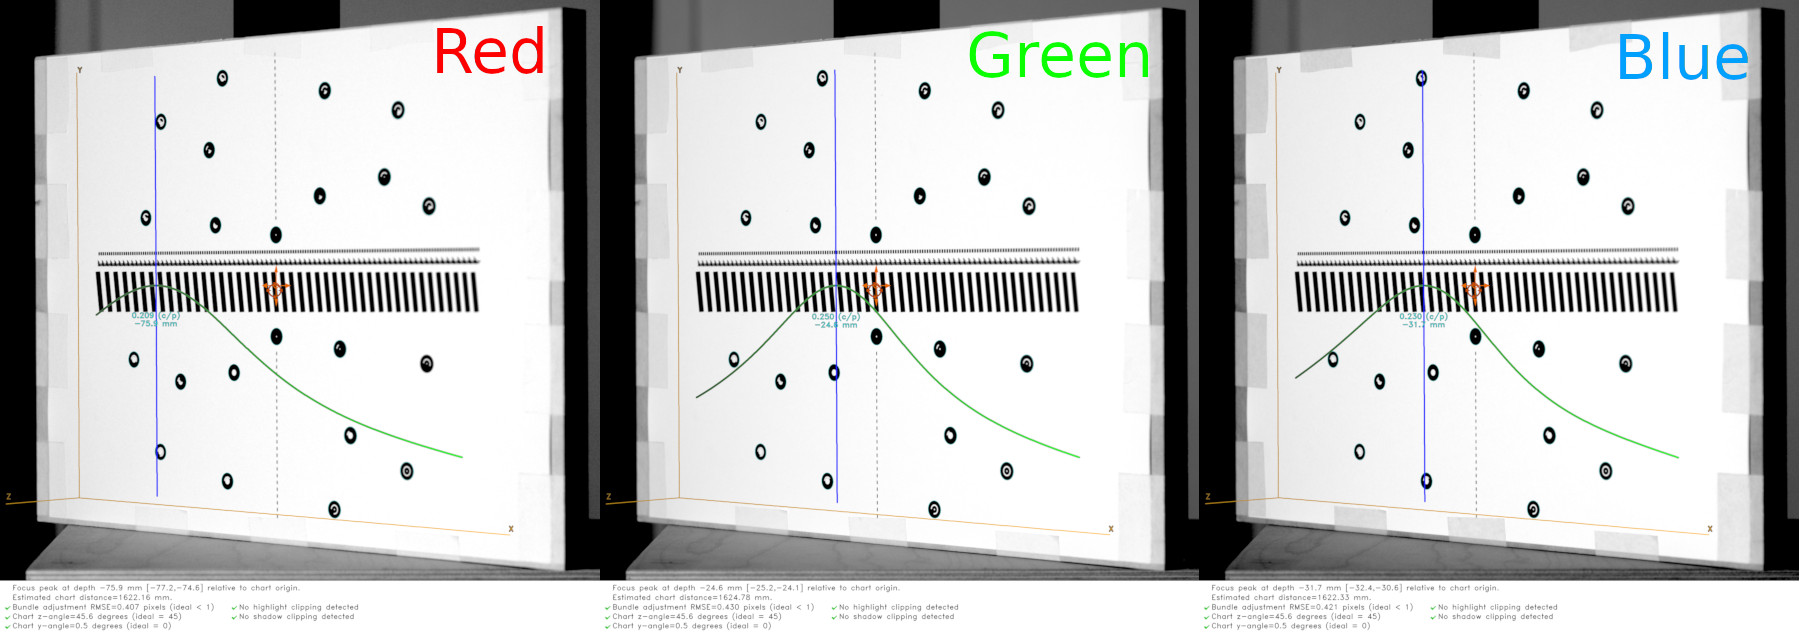
\includegraphics[width=0.95\textwidth]{figures/loca_example}
\caption{Example of longitudinal chromatic aberration. The same raw image
was processed by MTF Mapper three times, each time using only the indicated
colour subset of the sensor's Bayer filter. Notice how much
further back the red channel is focussed, relative to the green and blue
channels.}
\label{fig:loca_example}
\end{figure}

\subsection{Command line version outputs}
The bulk of MTF Mapper is implemented as a command-line utility, which makes
it suitable for scripted / batch operation. In fact, the only functionality
that is exclusively found in the GUI is the ability to automatically call dcraw to
convert raw camera image formats, and the ability to produce a plot of a
single SFR curve (see Section~\ref{sec:sfr_curve}).

In addition to producing all the graphical outputs described above, the
command-line utility can create a number of text files containing useful
measurements, e.g., a file giving the coordinates of an edge together with
its MTF50 value, or a file giving the coordinates of an edge together with
the full SFR curve data.

\newpage

\section{Getting started with the GUI}
\subsection{Main window}
After launching the GUI, you will be faced with a screen that looks like the
one portrayed in Figure~\ref{fig:sshot1}.

\begin{figure}[hb!]
\centering
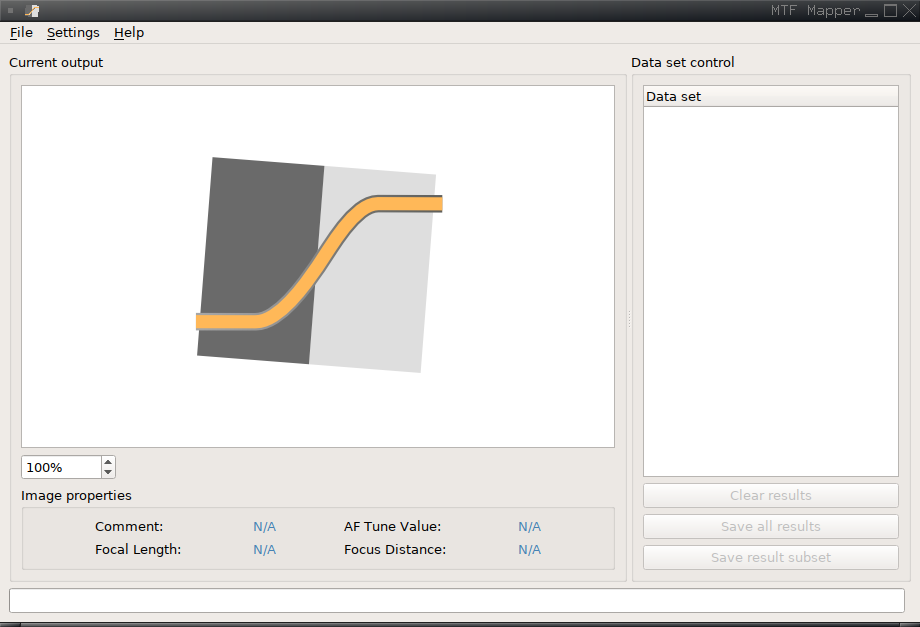
\includegraphics[width=0.85\textwidth]{figures/sshot1}
\caption{Screen shot of the MTF mapper gui}
\label{fig:sshot1}
\end{figure}


The first thing you probably want to do is open up a file (or multiple
files) by choosing \textsf{File/Open} from the menu bar. That gives you the
dialog depicted in Figure~\ref{fig:file_dialog}. Input files can be in a variety 
of image formats, including \texttt{.tif, .png, .jpg, .pgm}, 
or any raw format supported by \verb+dcraw+, including 
\texttt{.nef, .cr2, .pef, .arw, .orf, .rw2, .dng, .iiq, .mos}, and maybe more.

You may notice that there are two additional \textsf{Open} options, namely
\textsf{Open single edge image(s)}, and \textsf{Open Focus Position
image(s)}. These two entries are used to open very specific type of images,
which are discussed in Section~\ref{sec:single_roi_mode} and Section~\ref{sec:focus_distance_details}
respectively. Unless you are dealing with these specific image types, use
the plain \textsf{File/Open} option.

\newpage

I have drawn a red rounded rectangle on top of the screenshot to highlight
the output selection options --- these correspond loosely to the subsections
of Section~\ref{sec:overview} above.  There are several test charts (see
Section~\ref{sec:chart_types}) used by MTF Mapper, and not all of them will
work with all the output types.  Table~\ref{tab:combos} summarizes the
combinations that are supposed to work.

\begin{figure}[ht!]
\centering
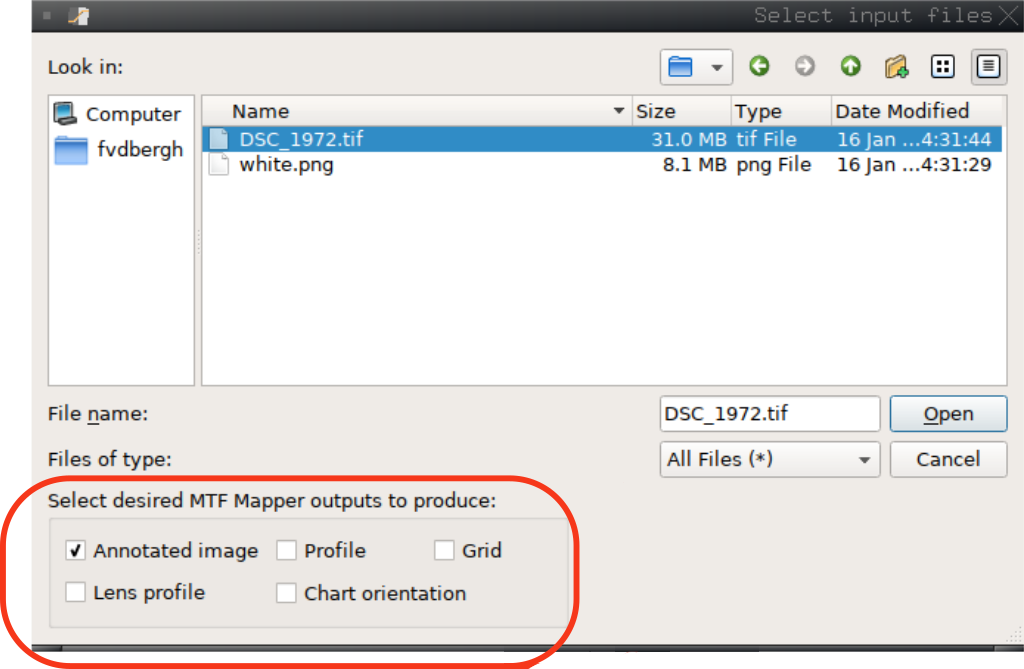
\includegraphics[width=0.65\textwidth]{figures/file_dialog2}
\caption{The File/Open dialog.}
\label{fig:file_dialog}
\end{figure}

\begin{table}[hb!]
\centering
\caption{Combinations of output types and chart types that should work}
\label{tab:combos}
\begin{tabular}{lp{10cm}}
\toprule
\bf Output type & \bf Compatible chart types \\
\midrule
Annotated image & lensgrid, grid, perspective, user defined \\
Profile         & perspective \\
Grid            & lensgrid, grid, perspective (not recommended), user defined \\
Lens profile    & lensgrid, grid (not recommended) \\
Focus position  & focus, mfprofile \\
Chart orientation & lensgrid, focus (not recommended) \\
\bottomrule
\end{tabular}
\end{table}

As you can see, the \textsf{Annotated image} output is the most flexible,
and will work not only with most of the MTF Mapper test charts, but also
with any user-provided test chart that contains black rectangles (actually,
most convex quadrilaterals) on a lighter background. It should work with ISO 12233:2014
E-SFR test charts (both standard and enhanced versions), but \emph{not} with
the older ISO 12233:2000 test charts, nor with DPReview's test charts. It is
possible to crop out sections of the latter two, which will work with MTF
Mapper (see Section~\ref{sec:single_roi_mode}).

\newpage

Ok, back to the file dialog. After you have selected your input file (or
multiple files with shift-click or ctrl-click), and
the desired output types, click the \textsf{Open} button to start
processing. You should see some entries appear in the \textsf{Data set}
tree-view list after a while. Each entry that successfully produced output
can be expanded by clicking on the symbol to the left of the entry (the
symbol is a triangle in QT5 on Linux). In Figure~\ref{fig:open_example2} I
expanded the entry of a file called \texttt{crop\_white} and selected the sub-entry
called \texttt{annotated} (highligthed by the red box).

\begin{figure}[bt!]
\centering
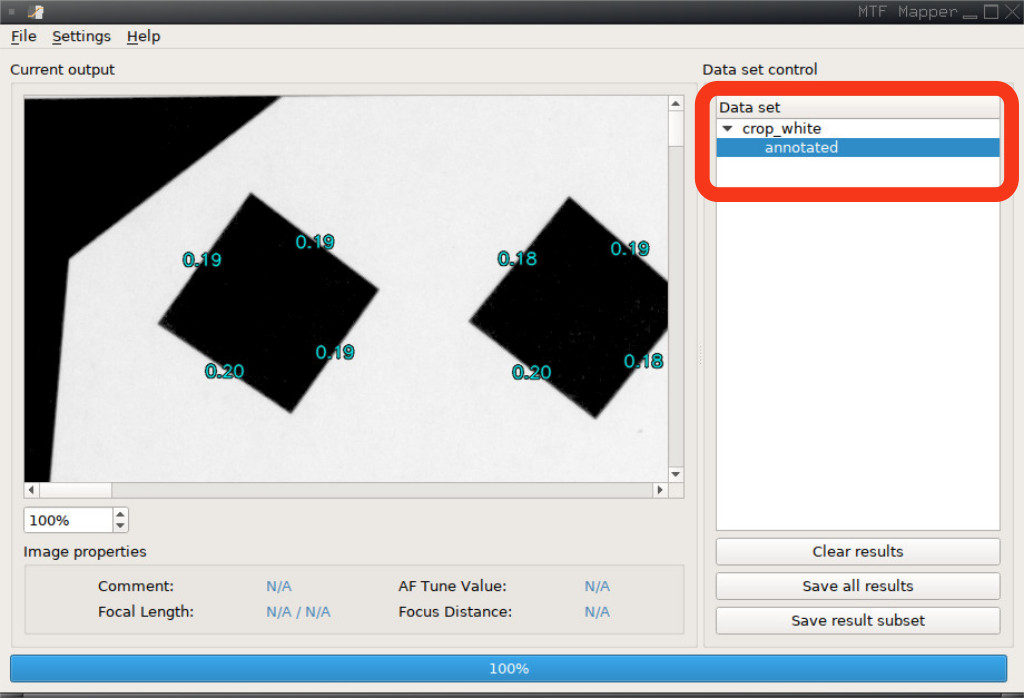
\includegraphics[width=0.85\textwidth]{figures/open_example2}
\caption{Selecting an output to view.}
\label{fig:open_example2}
\end{figure}

You can see the \textsf{Annotated} image output being shown in
the \textsf{Current output} panel; if the image dimensions exceed the window
size, then the initial display scale of the image
will be chosen so that one of the image dimensions fills the window
either horizontally or vertically.
You can drag the image in the output window to pan (while holding down the
left mouse button), or you may choose to use the scroll bars.
You may also use the mouse wheel to pan vertically, or hold down the shift
key while scrolling the mouse wheel to pan horizontally. You can zoom
in and out by holding down the control key while scrolling the mouse wheel,
but note that the maximum magnification factor is $2\times$. If the image is
smaller than the window size, zooming is disabled. Lastly, you can also zoom by
holding down the right mouse button while moving the mouse up/down, or by
clicking with any mouse button on the image to set the point around which
you want to zoom, followed by pressing the ``+'' or ``-'' keys on the keyboard.


At the bottom of the \textsf{Data set control} panel you will see three
buttons that can be used to either clear or save all the results currently
displayed in the \textsf{Data set} list.

The last panel of the main window can be found in the bottom-left corner:
the \textsf{Image properties} panel. Most of the fields are
self-explanatory, but I should note that these fields are populated purely
from the EXIF fields of your image, if present. In particular, the `Focus
Distance' property is that reported by the camera, and is not measured by
MTF Mapper.

One last thing to note: the size of the output plots/charts is determined by
the size of the main MTF Mapper window. If you maximize the window before
you open/process input files, then the plots shouls scale to fill the
window, which should help on very high resolution monitors.

\subsection{The preferences dialog}
\label{sec:settings}
The \textsf{Settings/Preferences} dialog is shown in
Figure~\ref{fig:settings}. The first panel we encounter (top left) looks
rather familiar; indeed, this \textsf{Output types} panel just a copy of the output
types options encountered in the \textsf{File/Open} dialog. The main
difference is that the output types selected in the \textsf{Preferences}
dialog are saved between MTF Mapper runs, and will be used to fill the corresponding
output type options in the \textsf{File/Open} dialog next time you run MTF
Mapper.

\begin{figure}[ht!]
\centering
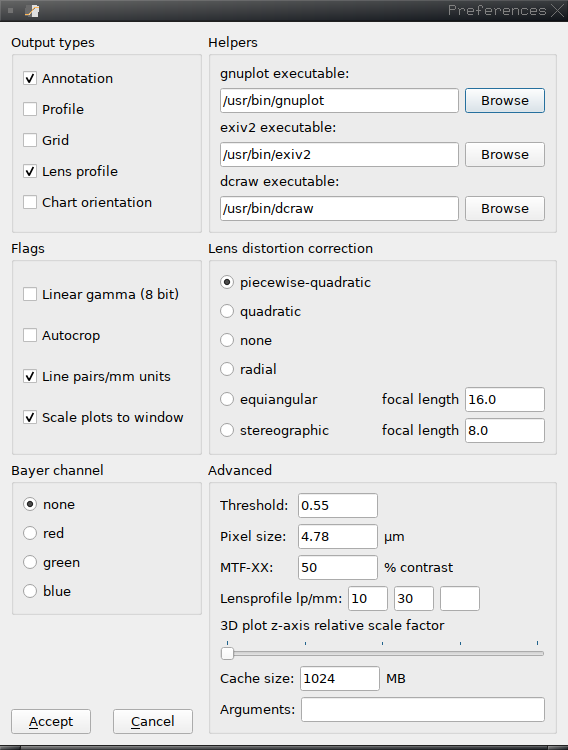
\includegraphics[width=0.65\textwidth]{figures/settings}
\caption{The preferences dialog.}
\label{fig:settings}
\end{figure}

The top-right panel, \textsf{Helpers}, is rather uninteresting unless you
want to use a custom version of \texttt{dcraw}. Normally, you can safely
ignore this panel.

The middle-left panel, \textsf{Flags}, contains a few optional flags that
can be set to alter MTF Mapper's behaviour. Briefly,
\begin{description}
\item[Linear gamma:] This option should be off by default. Most 8-bit images
(e.g., JPEGs) will be encoded with a particular gamma scheme; you can tick
this box if you are certain that your 8-bit input images are linear.
\item[Autocrop:] Automatically trim off a darker background border around your image
before the actual MTF Mapper processing begins. This is purely a speed
optimization that works well if the image circle of your lens is smaller
than your sensor. Which happens very rarely. Alternatively, if your test
chart does not fill the image, and the background behind your test chart is
dark enough, this option may also speed up processing a bit. If unsure,
rather leave it off.
\item[Line pairs/mm units:] This option (off by default) is used to switch
MTF Mapper's output units from the native cycles/pixel units to line
pairs/mm. Turn this setting on if you want your `Lens profile'
outputs to use the normal conventions, where resolution is expressed in
lp/mm. NB: if you turn on this option, then the `Pixel size' field in the
\textsf{Advanced} panel of the \textsf{Preferences} dialog must be set to
the correct pixel pitch of your sensor. If you use my default `Pixel size'
of 4.78 micron, you are only going to be happy with the result if you have a
Nikon D7000.
\item[Scale plots to window:] As previously mentioned, the varous
chart/plot outputs produced by MTF Mapper will be scaled to fill the main
window if this option is turned on (as it is by default). You can safely
leave this on.
\end{description}

The bottom-left panel, \textsf{Bayer channel}, is a lot more powerful than
its unassuming appearance might lead you to believe. If the `None' option is
selected, then your input image will be converted to a grayscale image
before the main MTF Mapper processing starts. Nothing (much) will happen if
your input image was already a grayscale image. Things get a little more
interesting if your input image is a raw camera format: with `None'
selected, your raw image will be demosaiced with the AHD algorithm
implemented in \texttt{dcraw} to produce a 16-bit linear RGB image, which
MTF Mapper will then promptly convert to a 16-bit linear grayscale image.
The conventional luminance conversion with a 0.299R + 0.587G + 0.114B weighing is
employed. The implication is that MTF Mapper will report on the MTF values
of the luminance channel of your RGB images if you leave the \textsf{Bayer
channel} option set to `None'.

If you choose a different \textsf{Bayer channel} option (`red', `green' or
`blue') \emph{and} your input image is a raw camera file, then two things
happen:
\begin{enumerate}
\item 
\texttt{dcraw} is instructed to produce un-demosaiced output, i.e., \texttt{dcraw}'s ``-d'' option, and
\item 
MTF Mapper will compute MTF values using \emph{only} the selected Bayer
colour subset. 
\end{enumerate}
The result of this is that \emph{no demosaicing algorithm interferes},
meaning that we can measure the MTF of the lens at the chosen wavelength
subset. (Strictly speaking, you would still have to remove the photosite aperture MTF
to really obtain the lens MTF, but you get the idea.)
This approach gives us the most accurate method of measuring effects like
longitudinal chromatic aberration, or any other phenomenon that could cause
the demosaicing algorithm to inadvertently mix the MTFs of the different
wavelength subsets (e.g., Red, Green, or Blue).


NB: Just keep in mind that only 25\% of the photosites of the sensor will be
red or blue, so it is prudent to use a longer edge for your MTF analysis.
Normally, I would recommend an edge length of at least 60 to 80 pixels for
grayscale images (or the luminance image MTF Mapper derives from a
demosaiced RGB image), but you should increase that (perhaps by using a larger
test chart) to at least 200 pixels for the red and blue Bayer channels.

NB: The default Bayer CFA pattern is RGGB.  If your sensor uses a different
pattern (rather unlikely) you can add \texttt{--cfa-pattern bggr} (or
whatever your pattern is) to the `Arguments' field in the \textsf{Advanced}
panel of the \textsf{Prefences} dialog. See Appendix~\ref{sec:manpages} for
all the supported CFA patterns.

The middle-right panel, \textsf{Lens distortion correction}, deals with
methods to work around lens distortion. Although MTF Mapper supports
multiple lens distortion correction methods, one should keep in mind that
the impact of lens distortion on slanted-edge MTF measurements is 
dependend on the length of the edges. Most MTF Mapper test charts feature
relatively small targets (the black rectangles / trapezoids), so the impact
of lens distortion will be relatively small. Having said that, the default
is for MTF Mapper to use a `piecewise-quadratic' to model each edge, which
should compensate for severe lens distortion on very large targets without
any meaningfull loss of accuracy. This method is suitable even when using
fisheye lenses. Section~\ref{sec:lens_distortion} covers this topic in more
detail.

The bottom-right panel, \textsf{Advanced}, covers a mixed bag of options.
\begin{description}
\item[Pixel size:]
The `Pixel size' field is almost self-explanatory; this field must be set to
your sensor's pixel pitch, expressed in micron (micrometre) units. This
field must be set to the correct value if the `Line pairs/mm units' option
is selected in the \textsf{Flags} panel; if that flag is disabled, then the
value of the `Pixel size' field is irrelevant, and will not be used by MTF
Mapper.

\item[Threshold:]
The most mysterious option in MTF Mapper is the `Threshold' field. To
understand what this parameter does, one has to consider how MTF Mapper
operates. The first step in MTF Mapper's processing is to threshold the
(grayscale) image so that the dark targets (e.g., black rectangles) are
separated from the lighter background of the test chart. This thresholding
step is locally adaptive, but it is still controlled by a threshold
parameter (between 0.0 and 1.0) to select just how dark an object has to be
relative to its surroundings. The default value of 0.55 should work well for
most properly-exposed images, provided that the test chart fills most of the
image.

But occasionally this will fail. Consider the case where you have set up
your test chart indoors, with the field of view adjusted to include the
whole test chart, with just a little bit of the background showing around
the chart. If this background scene happens to include a light source that
is much brighter than the white part of the test chart, then that light
source will `contaminate' the nearby part of the test chart, causing MTF
Mapper to not detect the black targets (rectangles) there. In other words,
the classic symptoms would be that only some of the black targets are
correctly annotated in the \textsf{Annotated image} output. The first (and
best) solution would be to not have a bright light source in the frame. 
The other potential solution is to decrease the `Threshold'
value until all the black targets are successfully detected. Starting from
the default value of 0.55, drop down to 0.4, 0.3, and maybe down to 0.2 if
necessary. 

You might wonder why I do not just set the default value to 0.3. Well, you
could have the opposite scenario where you have spurious dark objects in the
background that happen to be rectangular enough for MTF Mapper to detect.
The default value of 0.55 is a reasonable balance between these two
extremes, and works well enough until it doesn't, in which case you can
decrease it. Simple enough, right?

\item[MTF-XX:] By default, MTF Mapper will calculate MTF50 for most of its
outputs, such as the \textsf{Annotated image}, \textsf{Grid},
and \textsf{Profile} outputs. MTF50 is defined as the resolution (either in
lp/mm, or cycles/pixel) at which the MTF curve first reaches a value of
50\% contrast. This option allows you to specify a different target contrast
value in the range [10\%, 90\%], so you can calculate MTF20 or whatever you
desire. This affects all MTF Mapper outputs except the SFR curves and the
\textsf{Lensprofile} output.

\item[Lensprofile lp/mm:] By default, MTF Mapper will produce
\textsf{Lensprofile} plots at resolutions of 10 lp/mm and 30 lp/mm,
corresponding to the popular resolutions chosen by lens manufacturers. You can
override these default resolutions with this setting by specifying up to
three resolution choices in the range [1 lp/mm, 500 lp/mm]. Note that you
must have the `Line pairs/mm units' option checked in the \textsf{Flags}
panel for these values to be used, and the `Pixel size' field in the
\textsf{Advanced} panel must be set to the correct value.

\item[3D plot z-axis relative scale factor:]
Old versions of MTF Mapper (0.4.x and earlier) would plot the \textsf{Grid}
output (as illustrated in Figure~\ref{fig:surface_example}) scaled so that
the minimum MTF50 value would be treated as the zero reference for both the
z-axis height of the 3D MTF surface, and the colour scale for both the 3D
surface and 2D MTF image. This has the unintended consequence of magnifying
even tiny differences, should your lens behave very uniformly across the
field. It also means that it is hard to compare two different plots, since
the MTF50 scale can vary a lot between, say, f/1.4 and f/5.6.

In the 0.5.x MTF Mapper versions, the zero reference was always fixed at,
well, zero. The downside of this approach is that you could not see small
deviations in an otherwise very uniform performance across the field.

The solution, as implemented in versions 0.6.x upwards, is to leave the
choice to the user. Setting the `z-axis relative scale factor' slider all
the way to the left gives you the version 0.5.x beviour (zero is 0.0), and setting the
slider all the way to the right gives you version 0.4.x behaviour, like so:

\parbox{0.85\textwidth}{
\centering
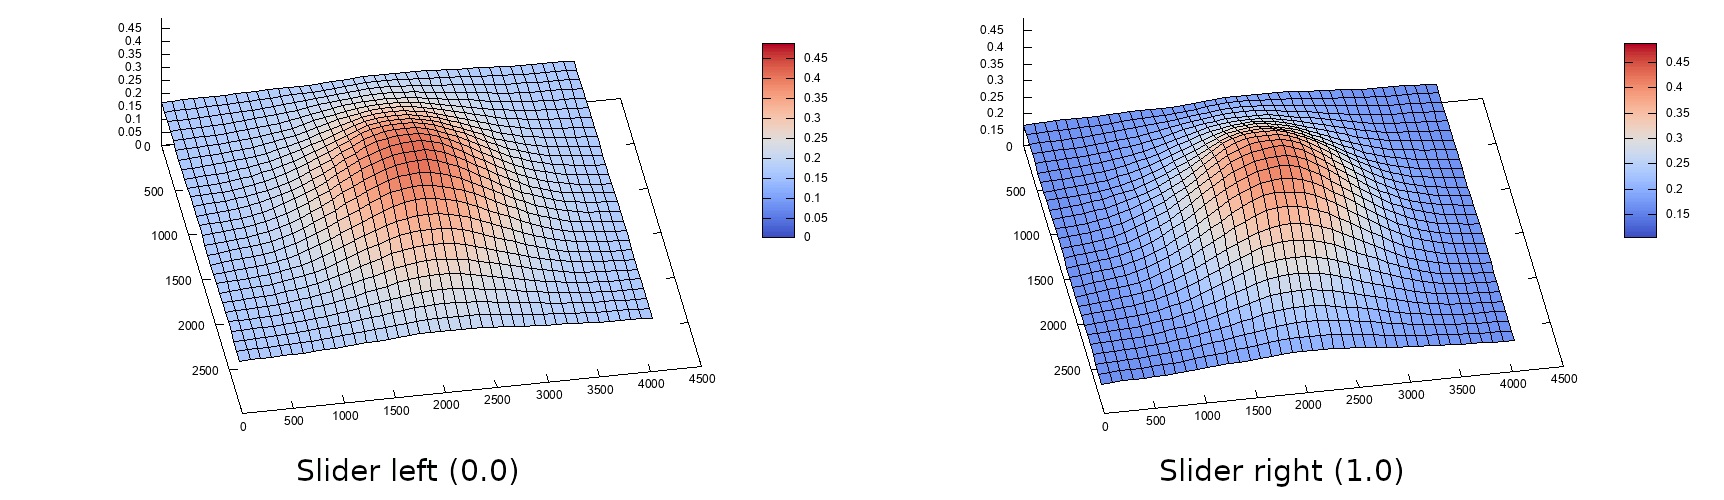
\includegraphics[width=\textwidth]{figures/z_axis_scale}
}

\item[Cache size:]
MTF Mapper will keep recently viewed images (including any output listed in
the \textsf{Data set} panel) in memory to avoid the delay in re-reading and
decoding the images when you rapidly switch between them. This parameter
controls how much memory (RAM) may be used for storing images; setting this
value to 1 MB (the minimum) effectively disables the cache. Adjust to taste.

\item[Arguments:]
This field gives you the opportunity to pass additional options to the MTF
Mapper command-line tool, thus you can obtain behaviour that is not
(currently) exposed in the \textsf{Preferences} dialog. See the MTF Mapper
command-line tool manual page (in Appendix~\ref{sec:manpages}) for a
comprehensive list of available options. For example, if you wish to turn
off the Savitzky-Golay filtering that MTF Mapper applies to the computed SFR
curves, you can add the \texttt{--nosmoothing} option to the `Arguments'
field.

If you find yourself using the `Arguments' field often, let me know and I
can try to extend the \textsf{Preferences} dialog to include the option you
require.

Note that from version 0.7.5 and upwards the contents of this field is saved
between MTF Mapper sessions. The contents of the `Arguments' field is not
sanitized, so it is possible to input invalid arguments, e.g.,
\texttt{--bogus}. If you entered such invalid arguments, the call to the MTF
Mapper command-line tool will fail, and you will get a pop-up dialogue that
will offer to reset the `Arguments' field. My advice is to accept this
offer.

\end{description}

\newpage

\section{Supported file types}
MTF Mapper is able to process a wide variety of image formats. The command
line utility can process at least \texttt{.tif}, \texttt{.png}, \texttt{.jpg},
\texttt{.ppm}, \texttt{.bmp} and \texttt{.pgm} files, and probably a few more formats
supported by OpenCV.

In addition to these, the MTF Mapper GUI adds support for automatic conversion of raw image
formats using \texttt{dcraw} to perform the conversion. At the time of
writing, the GUI will recognize the following raw file extensions:
\texttt{.NEF}, \texttt{.CR2}, \texttt{.ARW}, \texttt{.PEF}, \texttt{.IIQ},
\texttt{.MOS}, \texttt{.ORF}, \texttt{.RW2}, and \texttt{.DNG}. If you have
a specific format supported by \texttt{dcraw} that I missed, let me know and
I will add it!

As of version 0.6.15, MTF Mapper understands both ICC colour profiles, as
well as the two colour spaces supported by JPEG files via Exif tags (sRGB
and Adobe RGB). The slanted-edge method that MTF Mapper relies on only
works on `linear light' images, meaning that MTF Mapper will undo any
non-linear mapping (sometimes referred to as \emph{gamma correction}) associated with
the file format / colour space combination for \texttt{.tif} (TIFF) and
\texttt{.jpg} (JPEG) and \texttt{.png} (PNG) files. 
The following list summarizes how MTF Mapper deals with non-linear images:
\begin{enumerate}
\item
If you open a raw camera file with the GUI, then MTF Mapper will use
\texttt{dcraw} to produce a linear 16-bit RGB image. This is the most
accurate method. (Note: the command-line \texttt{mtf\_mapper} tool does not
automatically render raw camera files --- you have to use \texttt{dcraw} or
some other converter)
\item
If you open a TIFF file, a PNG file, or a JPEG file  (GUI or command-line)
with an embedded ICC profile, then MTF Mapper will convert the image to a
linear representation using the profile's Tone Reproduction Curve.  This
applies to both 8-bit and 16-bit TIFF and PNG files.
\item
If you open a JPEG file with some embedded Exif metadata, then MTF Mapper
will determine (well, guess) whether the JPEG file is in the sRGB or Adobe
RGB colour space, and apply the appropriate transformation to linearize 
the image.
\item
If your JPEG file has no Exif tags, or does not contain the Colour Space
tag, then MTF Mapper will assume the file is encoded in the sRGB colour space.
\item
If your image is in any other format (e.g., BMP or PNM), then MTF Mapper will 
assume that 8-bit images are encoded in the sRGB colour space (but you can
override this with the \texttt{-l} option), and that
16-bit images are linear.
\end{enumerate}

If you want to play safe, use a TIFF/PNG/JPEG file with an embedded ICC profile.
That takes care of linearizing the data. What about colour? Well, the
slanted-edge algorithm only operates on grayscale images, or one colour
channel at a time. MTF Mapper will transform an RGB image (after linearizing
the values if necessary) to a luminance image, i.e., it performs a CIE
RGB-to-XYZ conversion and keeps the Y channel.

If your image contains an ICC profile, then MTF Mapper will use the embedded
RGB-to-XYZ matrix which (according to the ICC specification) is already
adapted to a D50 illuminant. If your image is a JPEG file, then the
D50-adapted matrix for either sRGB or Adobe RGB will be used, as appropriate.
For all other file types, the D50-adapted sRGB matrix will be assumed.

\newpage

\section{Chart types}
\label{sec:chart_types}
MTF Mapper comes with a few custom test chart designs to fully realize its
potential. These charts can be partitioned into the \emph{perpendicular} and
\emph{$45^\circ$} families. All these charts can be generated using the
\texttt{mtf\_generate\_test\_chart} utility bundled with MTF Mapper. This is a
command-line only tool; see Appendix~\ref{sec:manpages} for a full
description of its options. The tool produces output charts in the SVG
vector format, which can be opened and edited with the Inkscape program (and
probably many others).

As an alternative, I keep a \texttt{.zip} file with a couple of charts
already converted to \texttt{.pdf} format on the MTF Mapper project on
SourceForge. Go to
\url{https://sourceforge.net/projects/mtfmapper/files/?source=navbar}, and
look for a file called \newline
\texttt{mtfmapper\_sample\_test\_charts\_xyz.zip}, \newline
where \texttt{xyz} will change whenever I update the archive.

\subsection{Perpendicular chart family}
These charts are designed to be used so that the test chart is parallel to
the camera's sensor, or equivalently, that the optical axis of the camera is
perpendidicular to the test chart.
\subsubsection{lensgrid}

\parbox{\textwidth}{
\centering
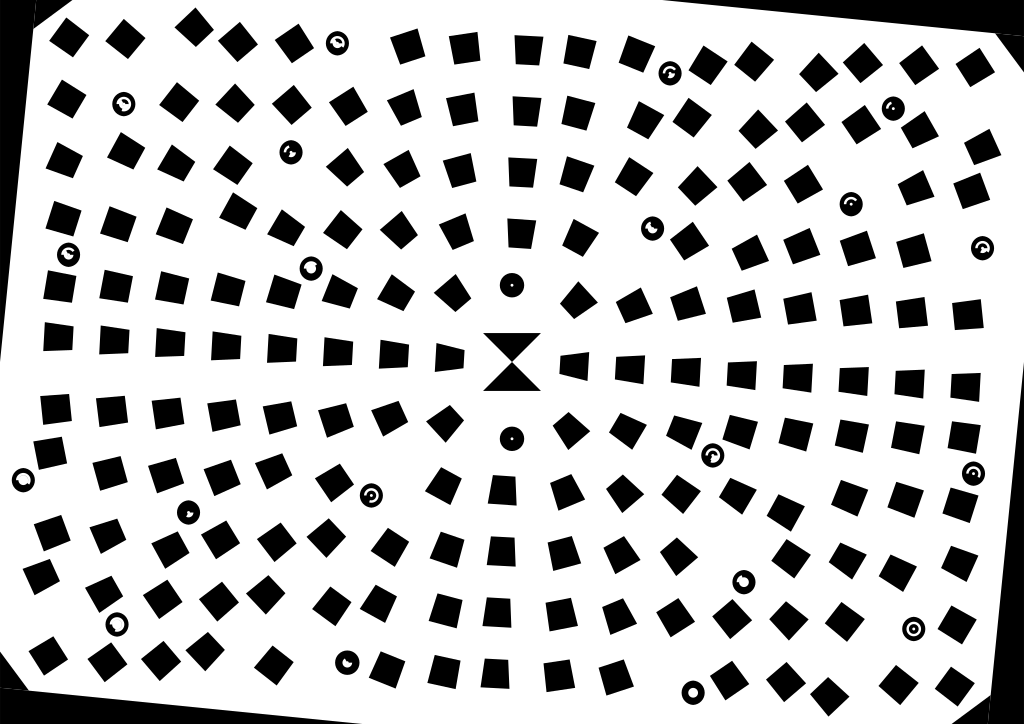
\includegraphics[width=\textwidth]{figures/chart_lensgrid}
}

\vspace{1ex}
This chart type is well-suited to most MTF Mapper output types, including
\textsf{Annotated}, \textsf{Grid}, \textsf{Lens profile} and \textsf{Chart
orientation}, \emph{but not} the \textsf{Profile} output type. The
particular shape of the targets, ranging from trapezoids to squares,
are specifically chosen to ensure that the edges are either purely radial or
tangential in their orientation, provided that the camera is centered on the
chart. Many thanks to Bernard Delley who proposed this type of chart on the
DP Review forums.

A quick word on slanted edge orientation is in order. If you have used
Imatest in the past, or you are familiar with the ISO 12233:2000 standard,
then you might wonder about the validity of MTF Mapper's test charts
containing edges that are clearly not placed at a $5^\circ$ angle. The short
version is that extensive testing using both simulated imagery and captured
imagery shows that the slanted edge method works just fine when applied to
edges that are not oriented at $5^\circ$ (see \cite{khom}, but I have also
independently performed these tests, e.g.,
\url{http://mtfmapper.blogspot.co.za/2015/06/anisotropy.html}).

In addition to the slanted edge targets, the chart also features a number of
circular fiducial patterns. These patterns are not used in MTF measurements,
but are used when automatic chart orientation measurement is performed
(see Section~\ref{sec:chart_orientation}). If you plan on using the chart
orientation feature, be sure to print the test chart at the correct size; if you closely
compare the A4 and A3 lensgrid charts (for example), you will notice that
the circular fiducial codes are different. I also recommend that you print
the charts without any `fit-to-page' options. The accuracy of the chart
orientation estimate depends on MTF Mapper being able to trust that the 
real-world distance between the circular fiducial patterns are correct for a
given chart size.

\subsubsection{grid}

\parbox{\textwidth}{
\centering
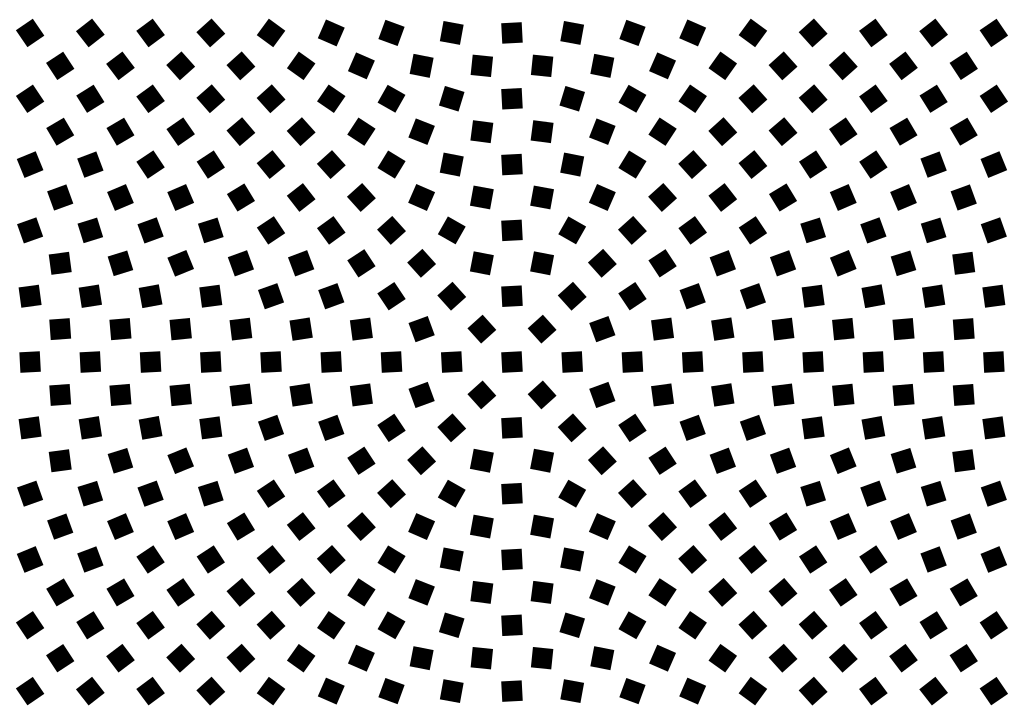
\includegraphics[width=\textwidth]{figures/chart_grid}
}
\vspace{1ex}

This chart type is provided for backwards compatibility, but I strongly
recommend the use of the \textsf{lensgrid} chart instead.

\subsection{$45^\circ$ chart family}
These charts are designed to be used such that the test chart is oriented at
a $45^\circ$ angle to the camera's optical axis (or sensor, for that matter)
in either the \emph{pitch} or \emph{yaw} directions. Actually, there is no
reason why these charts cannot be used at some other angle, e.g.,
$30^\circ$; rather consider that $45^\circ$ is a good starting point if you
do not know exactly how much depth-of-field to expect.

\subsubsection{perspective}
\label{sec:perspective_chart}

\parbox{\textwidth}{
\centering
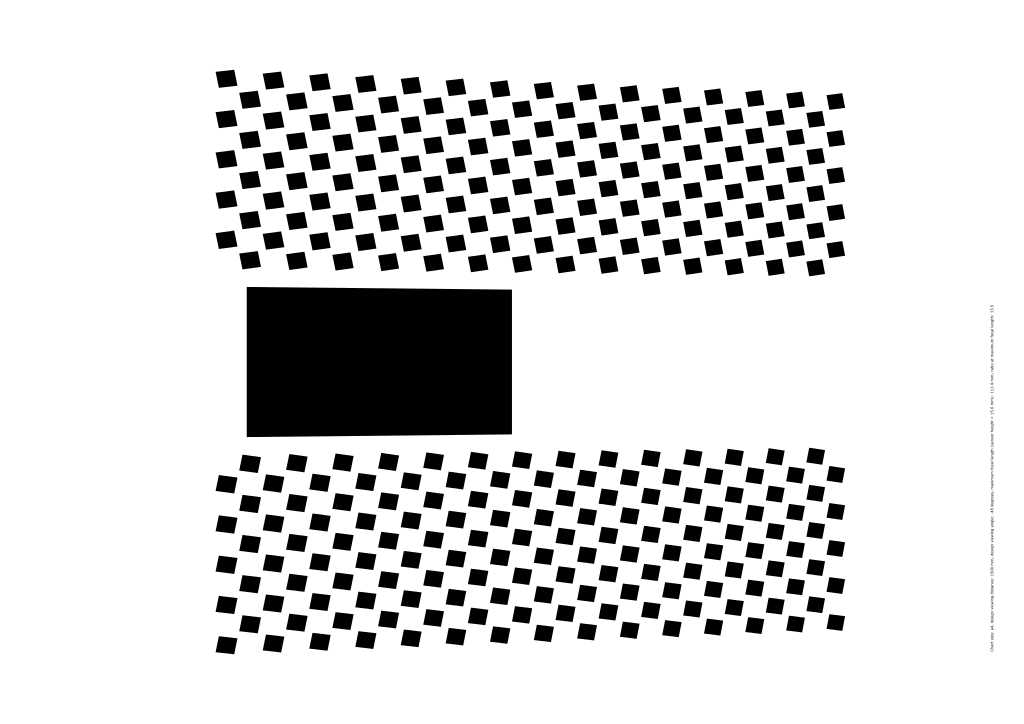
\includegraphics[width=\textwidth]{figures/chart_perspective}
}
\vspace{1ex}

The grandaddy of all MTF Mapper test charts, this chart is intended to be
used during autofocus callibration (see Section~\ref{sec:autofocus}). As
such, \textsf{Annotated image} and \textsf{Profile} (NB: \emph{not}
\textsf{Lens profile}) are the most useful MTF Mapper output types to use
with this chart.

\subsubsection{focus}

\parbox{\textwidth}{
\centering
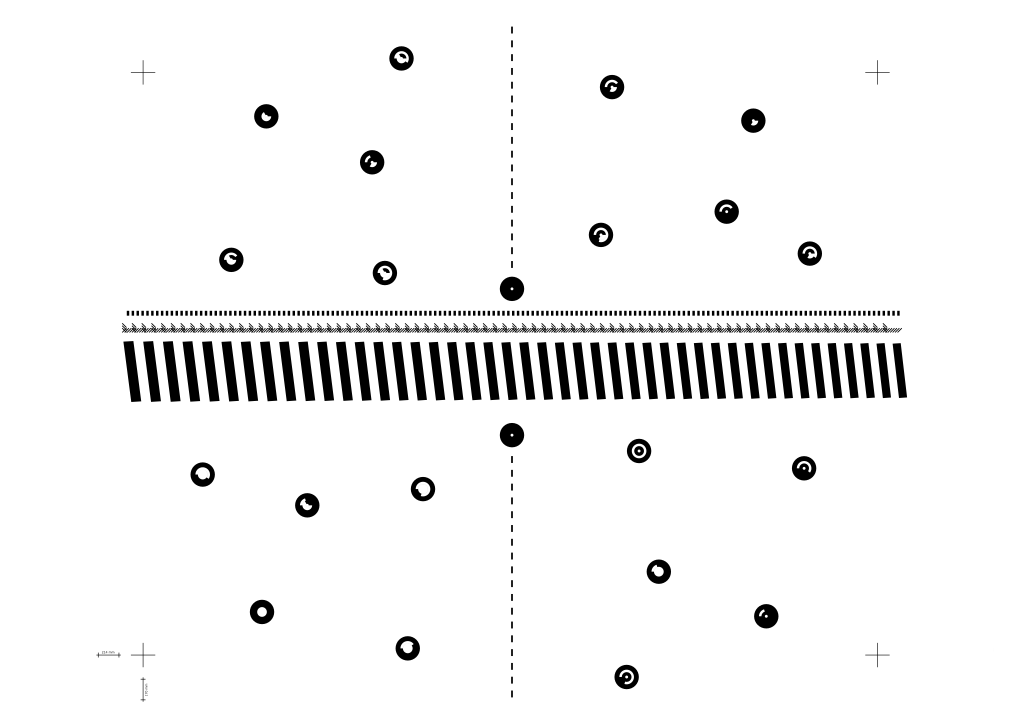
\includegraphics[width=\textwidth]{figures/chart_focus}
}
\vspace{1ex}

This chart type is intended to be used with the MTF Mapper \textsf{Focus
position} output type, which can only be selected by choosing 
\textsf{File/Focus Position image(s)} from the \textsf{File} menu in the GUI.
Trying to produce other MTF Mapper output types using
this test chart is not recommended.

\subsubsection{mfperspective}

\parbox{\textwidth}{
\centering
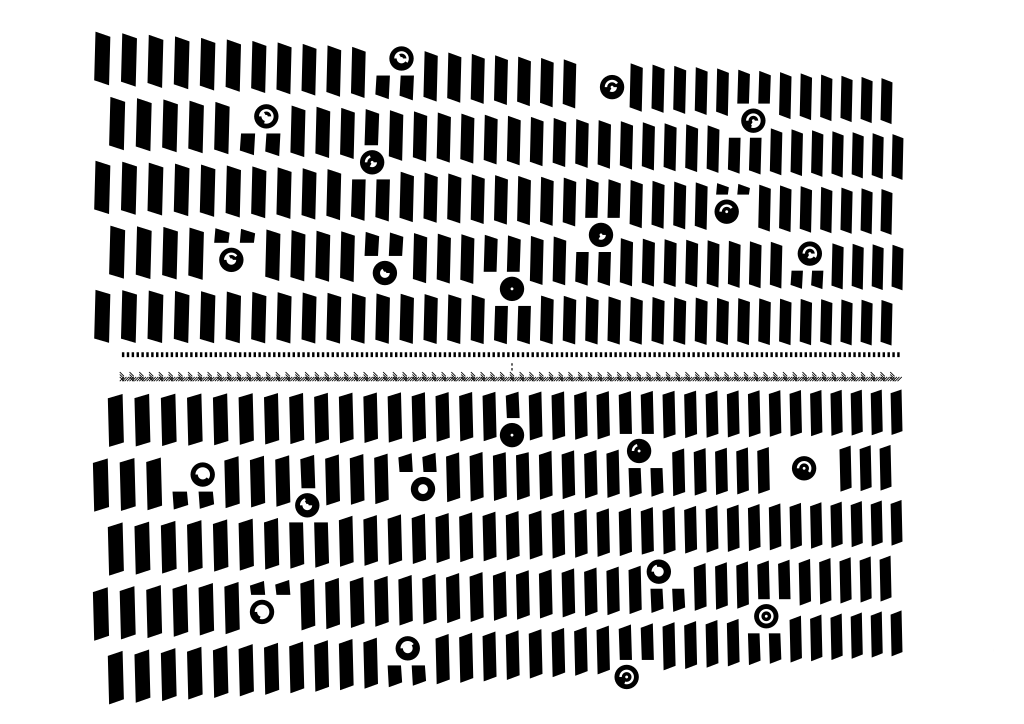
\includegraphics[width=\textwidth]{figures/chart_mfperspective}
}

This chart type is intended to be used with the MTF Mapper command-line
output option \texttt{--mf-profile}. 
Trying to produce other MTF Mapper output types using this test chart is not recommended.
At the time of writing, this chart and related output type are considered
experimental, and may potentially change in the future.

\newpage

\section{Additional details on how to use the output types}

\subsection{Lens profile MTF plots}
Section~\ref{sec:lens_profile} briefly introduced this output type. As a
first step, it is critical to ensure that the test chart is set-up to be
parallel to the image sensor, or equivalently, that the test chart is
perpendicular to the optical axis of the camera. The reason for this strict
requirement is clear when one considers how MTF Mapper derives the
\textsf{Lens profile} plots.

First, MTF Mapper assumes that the image centre is positioned to coincide
with the test chart centre (the bow-tie). Next, it averages all the MTF
measurements (contrast at a given spatial frequency) at the same radial
distance from the centre of the chart, grouping the edges into the sagittal
/ meridional orientations along the way. MTF Mapper also estimates the
spread of the measurements at that radial distance by computing the standard
deviation of the samples. Clearly, if the test chart is tilted badly in the
left-to-right direction you will end up averaging across measurements that
are in focus, behind the focal plane, and ahead of the focal plane. This
effect will become more pronounced towards the edges of the test chart.

\begin{figure}[!ht]
\centering
\begin{subfigure}[b]{0.5\textwidth}
    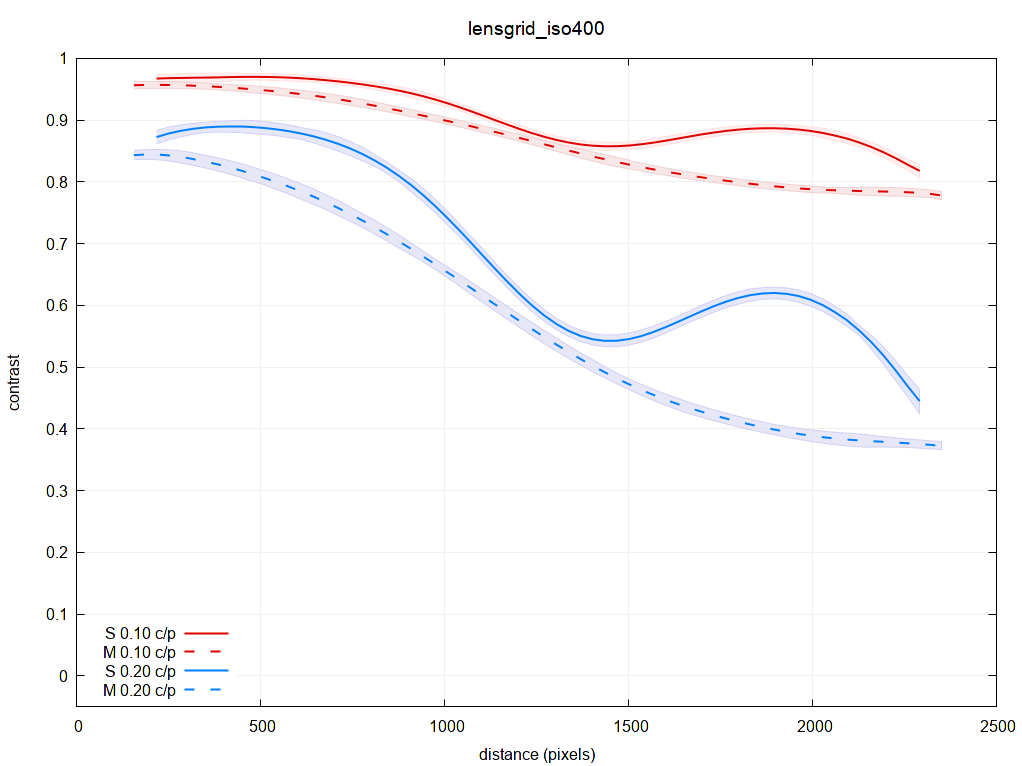
\includegraphics[width=\textwidth]{figures/lg_exmple_flat_lensgrid.png}
    \caption{Lens profile, no chart tilt}
\end{subfigure}
$\quad$
\begin{subfigure}[b]{0.25\textwidth}
    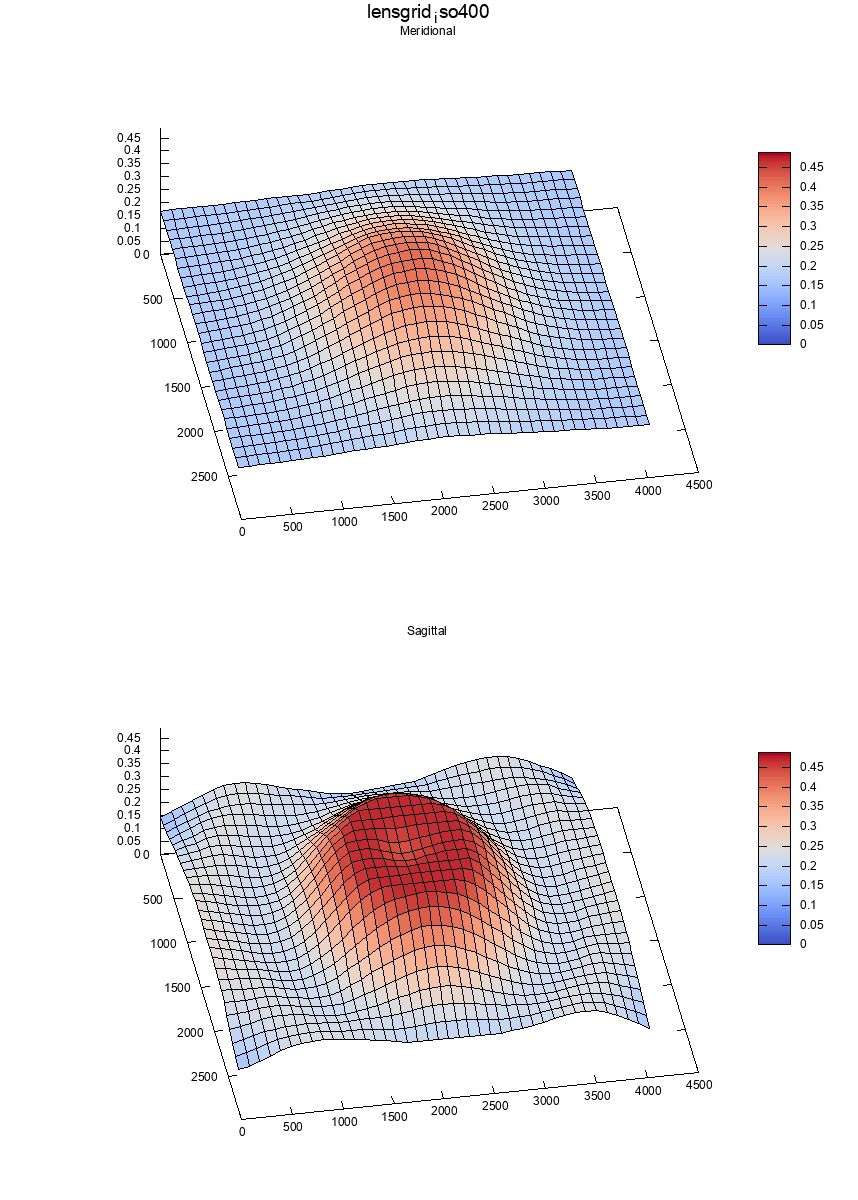
\includegraphics[width=\textwidth]{figures/lg_exmple_flat_surface.png}
    \caption{MTF50 surface, no chart tilt}
\end{subfigure}

\begin{subfigure}[b]{0.5\textwidth}
    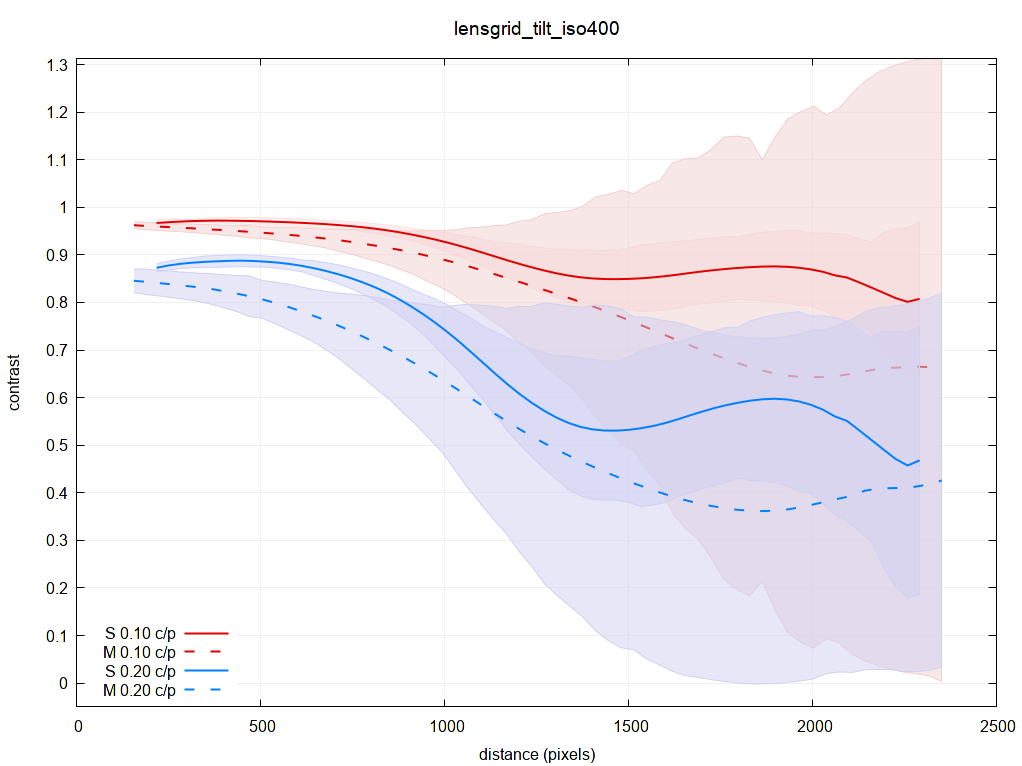
\includegraphics[width=\textwidth]{figures/lg_exmple_tilt_lensgrid.png}
    \caption{Lens profile, simulated chart tilt}
\end{subfigure}
$\quad$
\begin{subfigure}[b]{0.25\textwidth}
    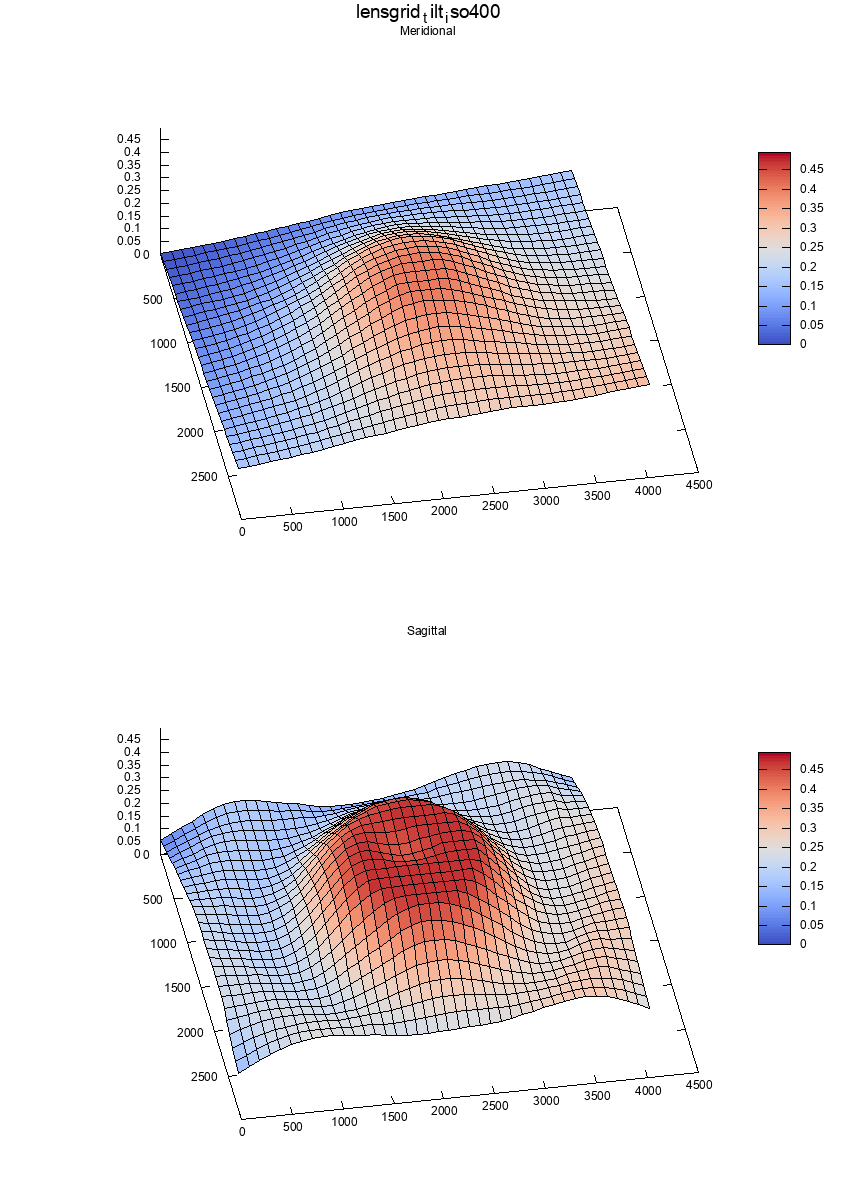
\includegraphics[width=\textwidth]{figures/lg_exmple_tilt_surface.png}
    \caption{MTF50 surface, simulated chart tilt}
\end{subfigure}
\caption{What happens when my chart is tilted slightly?}
\label{fig:lensgrid_tilt}
\end{figure}

Figure~\ref{fig:lensgrid_tilt} illustrates this effect using some simulated imagery.
Notice that although the general shape of the MTF curves have been preserved
(the solid and dashed lines in Figure~\ref{fig:lensgrid_tilt}(a) and (c)),
we see a massive increase in the observed spread of the measurements (the
red/blue shaded parts). The simulated amount of tilt is perhaps a little
excessive, but it should give you an idea of how to recognize tilt in a
\textsf{Lens profile} plot. Without further information (e.g., performing a
chart orientation measurement) it is not really possible to distinguish from
Figure~\ref{fig:lensgrid_tilt}(d) whether the chart is tilted (poor set-up),
or whether the lens has a tilted element.

Another important aspect when using MTF Mapper to generate \textsf{Lens
profile} plots is to choose the resolution units you want. By default, MTF
Mapper does not know the physical pixel pitch (size) of your sensor, and
this information is not reliably recorded in any EXIF tags. Thus, if you
want to produce a \textsf{Lens profile} plot using the typical 10 lp/mm and
30 lp/mm spatial resolutions, then you must set the `Pixel size' (in
the Advanced panel of the \textsf{Preferences dialog}) 
to the correct value, in micron. You must also tick the `Line pairs/mm units' box 
in the Flags panel.

\begin{figure}[!ht]
\centering
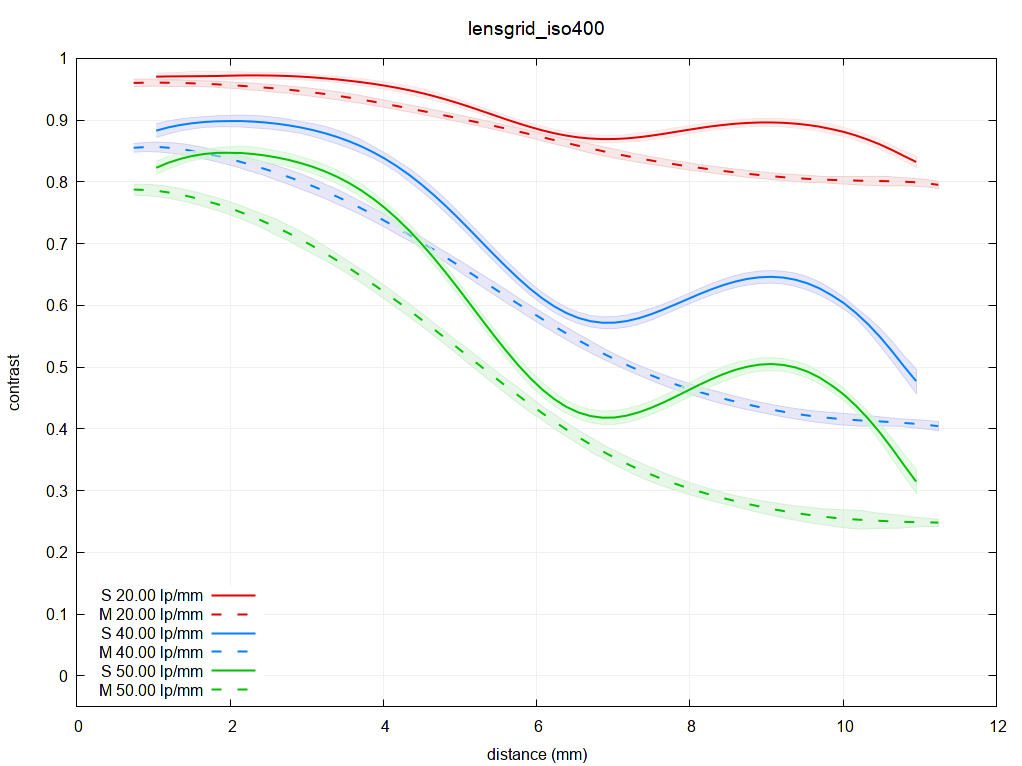
\includegraphics[width=0.75\textwidth]{figures/lens_profile_three.png}
\caption{You can specify up to three different spatial resolutions for
\textsf{Lens profile} outputs.}
\label{fig:lensgrid_three}
\end{figure}

If you want to plot the contrast at a different spatial resolution, e.g.,
50 lp/mm, then you can explictly tell MTF Mapper which resolution to use by
adding \texttt{--lp3 50} to the `Arguments' field of the
\textsf{Preferences} dialog. This will add a third curve for 50 lp/mm to the
output. You can override the default resolutions chosen for the first two
curves with by entering \texttt{--lp1 20 --lp2 40} into the `Arguments'
field. See Figure~\ref{fig:lensgrid_three}.

\subsection{Profile data sets / Autofocus fine-tuning}
\label{sec:profile_mode}
Using the \textsf{perspective} test chart illustrated in
Section~\ref{sec:perspective_chart}, 
the program will construct a profile such as the one shown in 
Figure~\ref{fig:sample_profile}. 
The chart should be photographed at a $45^\circ$ angle, preferrably at the specified
distance for that chart size. Each chart is optimised for a specific viewing distance to counter
the effects of perspective distortion, and the chart should be tilted such
that the `big end' of the chart is the one that is further away from the
camera.

\begin{figure}
\centering
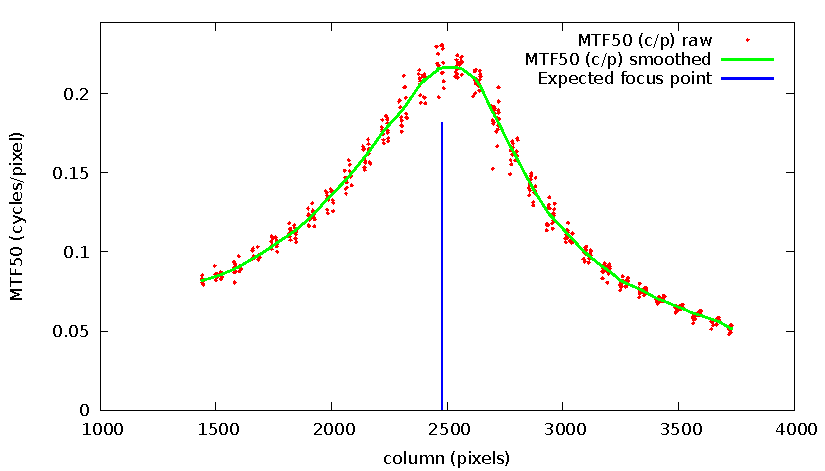
\includegraphics[width=0.95\textwidth]{figures/sample_profile}
\caption{Example of profile generated by MTF mapper.}
\label{fig:sample_profile}
\end{figure}

\begin{figure}
\centering
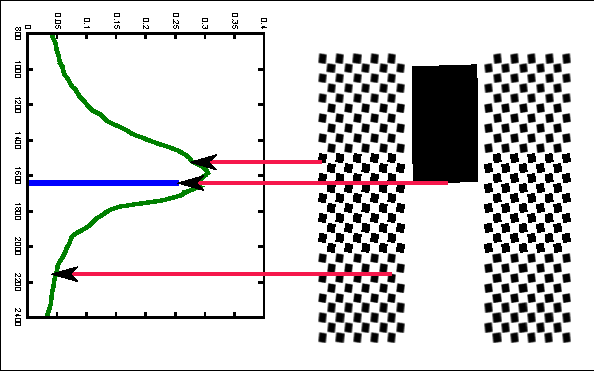
\includegraphics[width=0.8\textwidth]{figures/profile_construction}
\caption{How the profile is constructed: MTF50 values are collapsed
horizontally onto the $y$-axis to form the profile.}
\label{fig:profile_construction}
\end{figure}

The large central block in the test chart is called the reference block, and the edge of this block closest to the
centre of the chart is called the \emph{reference edge}.
The MTF50 values computed across the edges of all the blocks in the image
are projected onto the $y$-axis\footnote{MTF Mapper will auto-detect the
orientation of the image. For ease of discussion, this is called the
$y$-axis.} of the image, thus forming a new set of data
points of the form ($y$-value, MTF50 value). This process is illustrated in
Figure~\ref{fig:profile_construction}. The idea is that about half of the
chart will be in front of the plane of focus, and the other half behind. If
the depth of field is sufficiently shallow, then the closest and furthest of
the small blocks will be noticeably blurry. By projecting the measured
sharpness value (MTF50) of each block along horizontal lines
(Figure~\ref{fig:profile_construction}), we obtain a roughly bell-shaped
profile as shown in green on the left. The peak of this curve corresponds to the plane
of focus, and blocks that are further or closer than this plane are out of
focus to some degree. The blue line indicates the position of the
\emph{reference edge}.

A complete profile in its usual orientation is shown in 
Figure~\ref{fig:sample_profile}. The red dots represent individual MTF50
measurements, and the green curve is merely a smoothed representation of the
same data.

Generally, \emph{Profile} mode is only intended to be used to calibrate or
evaluate the autofocus sensor of a DSLR; the details of this process are
described in Section~\ref{sec:autofocus}. The objective is to adjust the
camera so that the blue line (reference edge, or focus position) lines up
with the peak of the green curve / red point cloud. If the blue line is far
from the peak, then you are experiencing either front- or back-focus. If
your chart was positioned at a $45^\circ$ angle so that the bottom edge 
was closer to you, then front focus would mean that the blue line appears to
the left of the peak in the green curve. This depends on the orientation of
the camera, though, so you may want to take a look at the \textsf{Annotated
image} (see Section~\ref{sec:annotated_images}) to orient yourself. The trick is to
remember that the peak in the green curve (or red point cloud) corresponds
to the \emph{actual} plane of focus, whereas the blue line corresponds to
where MTF Mapper \emph{assumes} you have placed the autofocus sensor when you
framed the shot.

\subsection{Plots of SFR curves (or MTF curves)}
\begin{figure}[!hb]
\centering
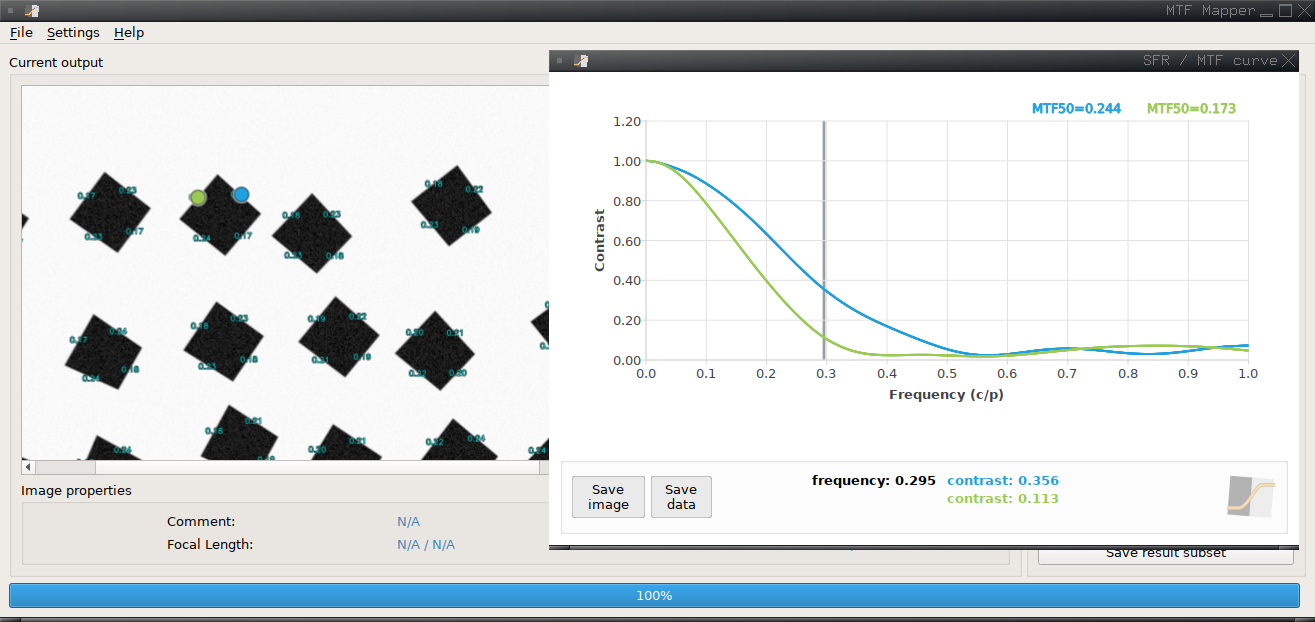
\includegraphics[width=0.85\textwidth]{figures/sfr_example}
\caption{Two edges have been selected. One is slightly out of focus, the other 
sharper. The pop-up window displays the SFR curves for both of these
edges by plotting contrast vs frequency. The two coloured dots drawn over
the selected edges in the annotated image correspond to the colours used 
to plot the SFR curves.}
\label{fig:sfr_example_repeat}
\end{figure}

A brief description of this output type is given in
Section~\ref{sec:sfr_curve}. The following points should be noted regarding
this output type:
\begin{enumerate}
\item 
Left-clicking on the MTF50 text labels (usually Cyan in colour) of the \textsf{Annotated image}
displayed in the \textsf{Current output} panel of the main MTF mapper will
cause a new SFR curve window to pop up, or will cause the current SFR curve
window to be replaced;
\item
Holding the shift key while left-clicking on the MTF50 text labels will
cause additional SFR curves to be added to the current SFR curve window. You
can select these additional edges from any of the \textsf{Annotated image}
outputs in the Data set list, e.g., you can select the same edge from two
images captured at different aperture values, or with different lenses, and
directly compare their SFR curves.

You could even process a single raw image three times with different Bayer
channels selected, and compare the SFR curves of the three channels 
using this technique.

If the window already contains three curves, shift-clicking will overwrite the
last curve added to the SFR curve window;
\item
MTF Mapper draws coloured dots on the \textsf{Annotated image}
output to indicate which edges are being plotted in the SFR curve window;
\item
The SFR curve window supports the display of the full SFR curve, i.e., by
adding the \texttt{--full-sfr} option to the `Arguments' field of the
\textsf{Preferences} dialog \emph{before opening the input files for
processing}, the SFR curve will be displayed up to 2.0 cycles/pixel (the
default is 1.0 cycles/pixel);
\item
The `Save data' button of the SFR curve window (see
Figure~\ref{fig:sfr_example}) will save the currently displayed SFR curves
to a CSV file. If multiple curves are displayed, then they will form
additional columns in the output CSV file;
\end{enumerate}

\subsection{Checking test chart orientation}
\label{sec:chart_orientation_details}
A brief overview of this output type is presented in
Section~\ref{sec:chart_orientation}. 
A close-up of the output image is shown in Figure~\ref{fig:chart_orientation_example_rep}.
The centre of the printed test chart is defined as the point where the tips
of the two black triangles touch, in the shape that resembles a bow-tie.
After successfully extracting the test chart coordinate information from the
circular fiducial patterns, MTF Mapper will visualize the chart origin by drawing
an orange `compass rose' on top of the output image.

The second important marker symbol, a red circle with four inwards-pointing
triangles, is drawn at the location of the image sensor centre (see
Figure~\ref{fig:chart_orientation_example_rep}). This marker should ideally
be close to the orange compass rose, thus serving as a visual indicator of
how well the test chart was centered in the camera frame, but it does not
have to be spot-on.


\begin{figure}[!ht]
\centering
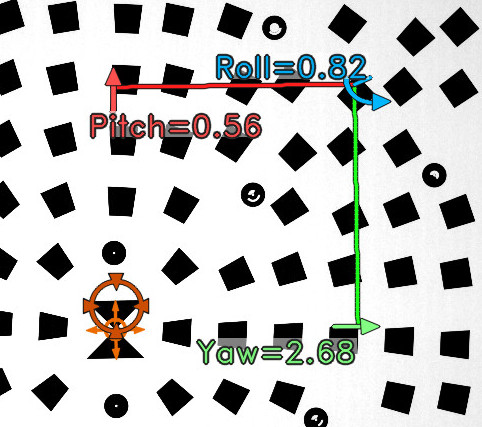
\includegraphics[width=0.75\textwidth]{figures/orientation_example_closeup}
\caption{A close-up of the chart orientation output. This is a crop of
Figure~\ref{fig:chart_orientation_example}.}
\label{fig:chart_orientation_example_rep}
\end{figure}

The three Tait-Bryan orientation angles (yaw, pitch and roll) are also
rendered in colour on top of the output image. Each rotation is indicated by
a short arc ending in an arrow; this arrow points in the direction of the
observed rotation, so corrections must be applied in the opposite direction.
Aim to reduce all three the angles to below $1^\circ$.

Note that MTF Mapper can only estimate the chart orientation accurately if
it knows the \emph{focal ratio} of the camera. The focal ratio is simply
defined as focal length (in mm) divided by sensor width (in mm). MTF Mapper
will attempt to extract this information from the EXIF tags in the image,
but not all camera hardware will provide the relevant tags. In that case, it
is necessary for the user to provide this information using the
\texttt{--focal-ratio} option, which can be added to the `Arguments' field
of the \textsf{Preferences} dialog of the GUI.

Keep in mind that the chart orientation measurement is based on the
geometrical projection of the lens, not on MTF or sharpness. In other words,
if your camera sensor is tilted with respect to your lens mount (someone
dropped a camera, perhaps), then the chart orientation measurement provided
by MTF Mapper will allow you to orient your camera such that the sensor is
parallel to the test chart. By looking closely at the \textsf{Grid} output,
you should be able to see whether the plane of best focus is still parallel
to the test chart --- if not, then either your sensor or lens mount is
tilted, or your lens contains a tilted element. Repeating with a second lens
should reveal the truth.

\subsection{Focus distance-, focus shift-, or LoCA measurement}
\label{sec:focus_distance_details}
A brief description of the \textsf{Focus position} output type can be found in
Section~\ref{sec:focus_distance}; this section covers some important
details. Note that since MTF Mapper 0.6.20 this output type can only 
be produced by opening the files using \textsf{File/Open Focus Position
image(s)}, but in older versions a regular checkbox existed to select this 
output type.

\begin{figure}[ht!]
\centering
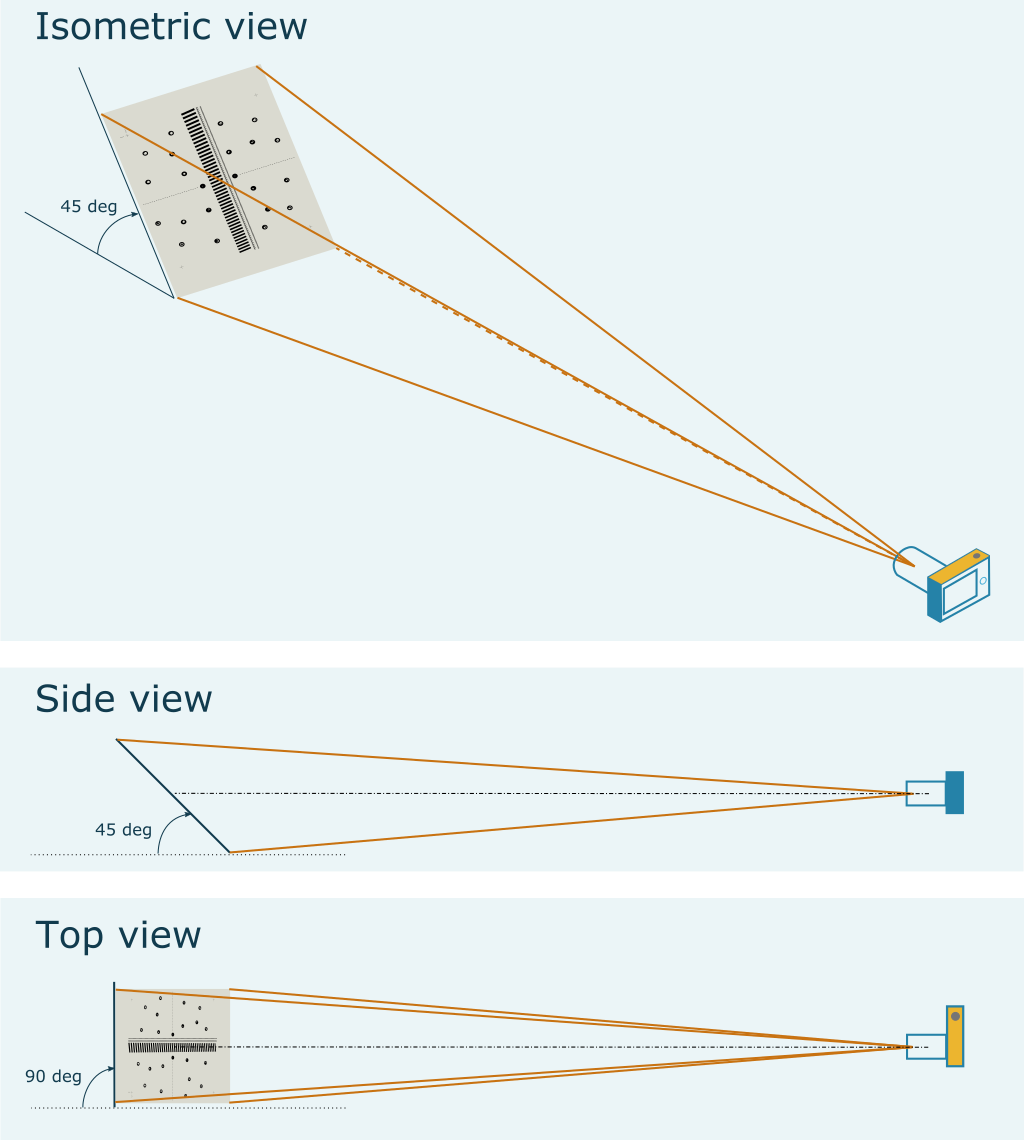
\includegraphics[width=0.65\textwidth]{figures/focus_chart_diagram}
\caption{How to set up the chart relative to the camera.}
\label{fig:focus_diagram}
\end{figure}

The \textsf{focus} test chart is intended to be used as illustrated in
Figure~\ref{fig:focus_diagram}. MTF Mapper measures the focus position
relative to the centre of the chart, meaning that focus should be set (using
manual focus) to the section of the chart indicated in
Figure~\ref{fig:manual_focus_position}. You will notice that there are some
chevron-like patterns down the centre of the chart to facilitate manual
focusing; Live View focussing with magnification is recommended.

\begin{figure}
\centering
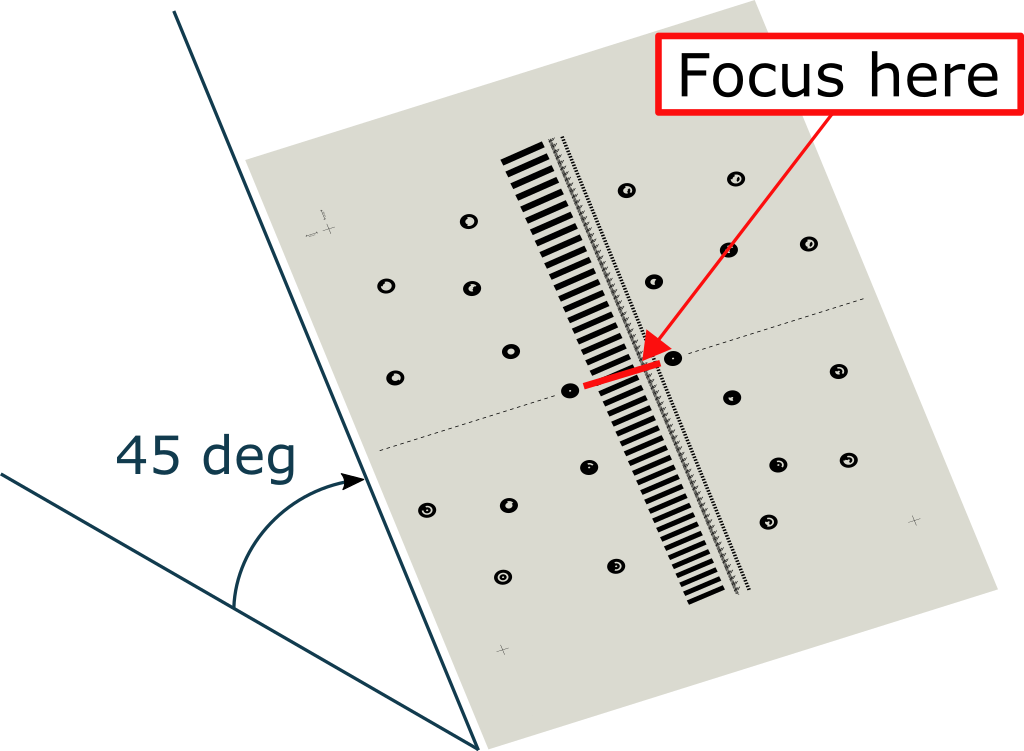
\includegraphics[width=0.65\textwidth]{figures/manual_focus_position}
\caption{Focus where the red line shows.}
\label{fig:manual_focus_position}
\end{figure}

The first experiment that you can perform with this MTF Mapper feature is to
measure your own manual-focus accuracy. You capture a number of shots,
resetting focus to infinity beforce re-focusing each time, then use MTF Mapper to measure how
close to perfect focus you came in each shot.
Figure~\ref{fig:manual_focus_reading} highlights the \emph{focus error} that you are
looking for: the difference between the point of peak sharpness and the
intended focus position (the centre of the chart). You can tabulate these
values using your favourite spreadsheet to see how repeatable your manual focus technique is.

\begin{figure}
\centering
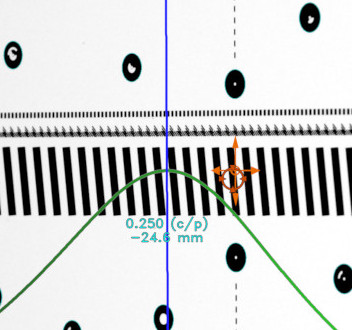
\includegraphics[width=0.5\textwidth]{figures/manual_focus_reading}
\caption{The focus error is the value $-24.6$ mm printed in Cyan on top of
the chart image.}
\label{fig:manual_focus_reading}
\end{figure}

The red circle with the four inwards-pointing triangles that can be seen in 
Figure~\ref{fig:manual_focus_reading} is a visual indication of the centre
of the image, and thus the sensor. This marker should  perferably coincide
with the centre of the chart (indicated with the orange compass rose); it
just makes things easier if you aim the camera so that the centre of the
sensor lines up with the centre of the test chart, and then you try to place
the focus on the centre of the test chart.

So how does this MTF Mapper output type work? Well, the wide black bars that
run down the centre of the chart are used to measure MTF50, but only on the
wide edges of the bars. Because the camera is centered on the chart, these
measurements are all in a purely meridional orientation, and the tilt of the
chart ensures that each bar is at a slightly different distance from the
camera. Actually, MTF Mapper takes multiple MTF measurements along each of
the long edges of these bars to ensure good depth coverage.

Once all the measurements are collected, MTF Mapper fits a rational
polynomial function to the MTF50 vs distance samples; this is the green
curve seen in Figures~\ref{fig:manual_focus_reading} and
\ref{fig:focus_example}. This green curve is a direct visualization of a
Depth Of Field (DOF) curve, but using MTF50 as the sharpness criterion instead 
of using a circle of confusion. Although MTF Mapper projects this
green curve back onto the image of the test chart, the actual measurements
are available in a true depth scale (distance from camera) in millimetres.

Note that you can use the \textsf{Focus position} output of MTF Mapper with
a normal demosaiced image, i.e., \textsf{Preferences}/`Bayer
channel' set to `None', with raw images or JPEGs, to perform the focus
position measurement on the luma component of your image. This should
correspond to your normal visual perception of sharpness in the image.

\subsubsection{Focus shift measurement}
You can measure the amount of focus shift your lens experiences on stoping
down directly in object space (or the field, if you prefer that term). 
First, use manual focus at your camera's focusing aperture (usually the
maximum aperture of the lens) to adjust your focus until the \emph{focus
error} (see Figure~\ref{fig:manual_focus_reading}) is small, say, below 10
mm.  Then stop down the lens \emph{without adjusting focus}, and capture
another shot.  The difference between the \emph{focus error} of the
wide-open shot and the stopped down shot will give you a direct measurement
of the amount of focus shift. This measurement will most likely depend on
the overall distance from your camera to the test chart, so choose a chart
size that will work at the camera-to-chart distance you intend to use the
lens at most often.

If you find that the focus shift is so extreme that the focus position moves
completely off the test chart, then you could try to tilt the test chart
further away from parallel to the sensor. This should increase the depth
range spanned by the chart, and hence bring the focus shift into range. The
downside of this would be a slight decrease in depth measurement resolution.

\subsubsection{Longitudinal Chromatic aberration measurement}
Similarly to the above recipe for measuring focus shift, first adjust your manual
focus position until the \emph{focus error} (see Figure~\ref{fig:manual_focus_reading})
is small. Then use the \textsf{Preferences}/`Bayer
channel' settings to choose the red, green and blue channels, each time
using \textsf{File}/`Open' to process \emph{the same} raw input
image in turn. Figure~\ref{fig:loca_example_rep} illustrates the results of
such an experiment where we can clearly see that the red channel focuses
far behind the blue and green channels --- this happens to be a Nikkor 50 mm
f/1.8 AF-D lens shot at f/2.8.

\begin{figure}[!ht]
\centering
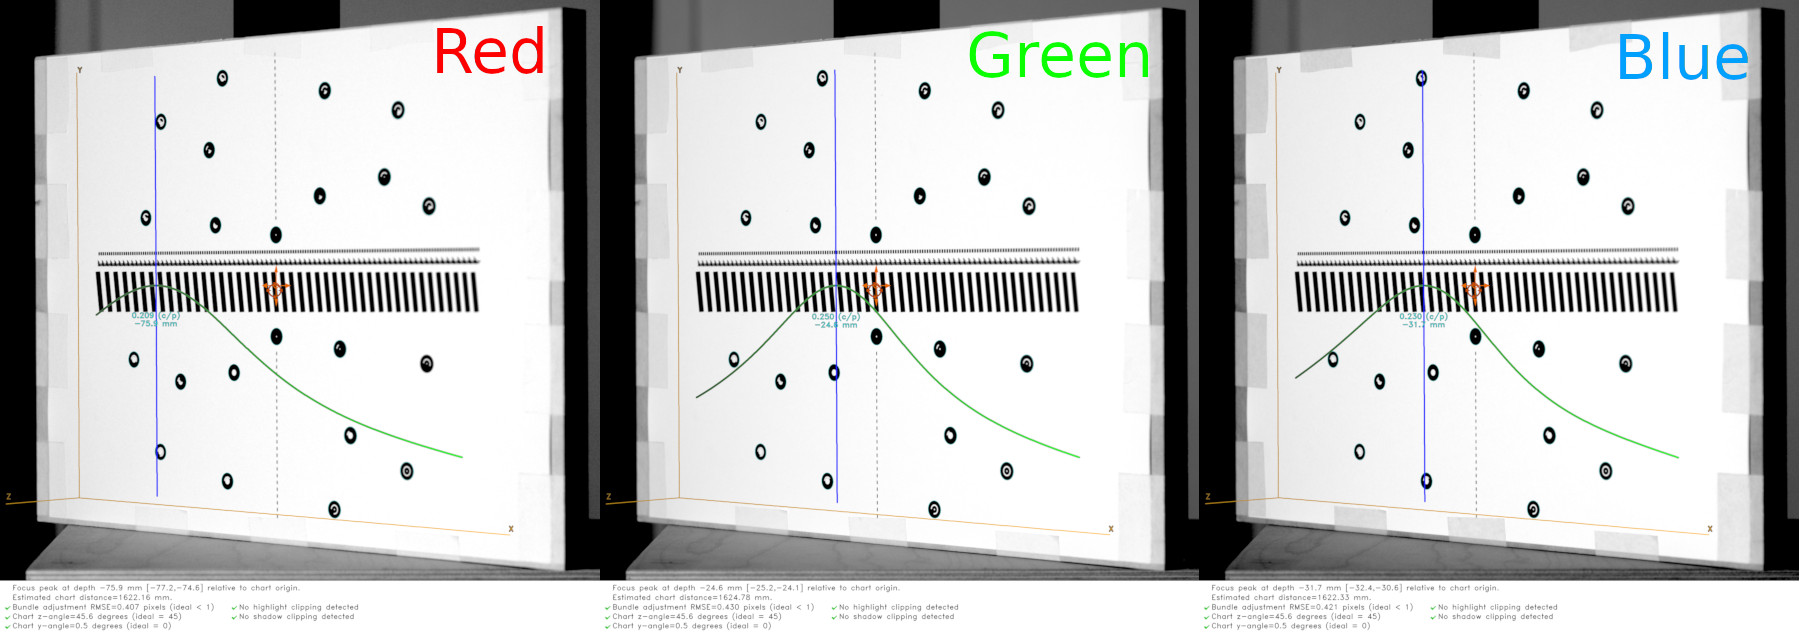
\includegraphics[width=0.95\textwidth]{figures/loca_example}
\caption{Example of longitudinal chromatic aberration.}
\label{fig:loca_example_rep}
\end{figure}

\newpage 

\subsection{Useful command line outputs}
Although this guide is focused on the features offered by the GUI, it seems
like a good place to document the most useful output offered to command-line
users of MTF Mapper. The option in question is ``-q'', which would be
invoked as \verb+mtf_mapper input.tif out -q+. This output option produces
SFR data, MTF50 data, and lens distortion data, distributed over three
output files:
\begin{description}
\item[\texttt{edge\_mtf\_values.txt}:]
Each row of the \texttt{edge\_mtf\_values.txt} file contains six space-separated columns:
\emph{block\_id} \emph{edge\_x} \emph{edge\_y} \emph{mtf50} \emph{corner\_x}
\emph{corner\_y}. The \emph{block\_id} can safely
be ignored (it depends on the order in which target squares were processed).
The pair (\emph{edge\_x}, \emph{edge\_y}) denote the pixel coordinates of the centroid
of the edge, and \emph{mtf50} is the MTF50 value in cycles per pixel (default),
or in lp/mm if the \verb+--pixelsize+ option was specified. Lastly, the pair
(\emph{corner\_x}, \emph{corner\_y}) denote the pixel coordinates of the corner of the
target (black square) associated with this edge, and can be safely ignored.

\item[\texttt{edge\_sfr\_values.txt}:]
The format of the \texttt{edge\_sfr\_values.txt} file is similar: each row starts with
five columns: \emph{block\_id} \emph{edge\_x} \emph{edge\_y}
\emph{edge\_angle} \emph{radial\_angle}, followed by 64 more floating point values denoting the SFR. 
The \emph{edge\_angle}
column denotes the orientation of the edge relative to the image
rows/columns, modulo 45 degrees. This angle should perferably be at least 2
degrees but less than 44 degrees for best results. The fifth column,
\emph{radial\_angle}, is just the angle of the radial line from the image centre
to the edge centroid, thus it can be used to determine whether an edge is in
a sagittal or meridional orientation with respect to the image centre, which
is assumed to be centered on the test chart.

The SFR part (the last 64 values on each line of
\texttt{edge\_sfr\_values.txt}) represents the contrast values of the SFR (or MTF, if you prefer) sampled at
spatial frequencies of i/64 cycles per pixel for i from 0 to 63 inclusive.
You can readily transform these frequencies to another linear resolution
scale, e.g., if your sensor's pixel pitch is 4.78 micron, then the
frequencies can be scaled so that i/$64\times1000/4.78$ gives you a resolution
scale in line pairs per mm.


If you use the \verb+--full-sfr+ option together with \verb+-q+, the SFR component of
each line of \texttt{edge\_sfr\_values.txt} will comprise 128 values (rather than 64), 
and the corresponding spatial frequencies are i/64 cycles per pixel for i from 0 to 127 inclusive.

\item[\texttt{edge\_line\_deviation.txt}:]
Each row of the \texttt{edge\_line\_deviation.txt} file contains six space-separated columns:
\emph{block\_id} \emph{edge\_x} \emph{edge\_y} \emph{slope} \emph{rise}
\emph{run}. The first three, \emph{block\_id} \emph{edge\_x} \emph{edge\_y},
have the same meaning as in the other files (e.g.,
\texttt{edge\_mtf\_values.txt}). The interesting columns are, of course,
\emph{slope}, \emph{rise} and \emph{run}. Figure~\ref{fig:line_deviation}
illustrates what these values mean. The figure shows the curvature of an
actual edge processed by MTF Mapper; the purple `+' symbols are individual
measurements of the edge location (in the v-axis) along the length of the
edge (the u-axis), and are clearly affected by image noise.
It helps to keep the scale of the axes in mind: the \emph{rise} value is
only 0.06 pixels, with the \emph{run} dimension weighing in at 70 pixels. 
The green parabola represents a curve fitted to the raw
data. As shown in the figure, the \emph{run} and \emph{rise} parameters are
measured on the fitted parabola, rather than the raw data points, to avoid
the image noise. The \emph{slope} value (and fourth column of
\texttt{edge\_line\_deviation.txt}) is just the ratio
\emph{rise}/\emph{run}.

I have yet to perform a calibration experiments to determine the critical
values of the parameters which would partition edges into \emph{curved} and
\emph{not-really-curved} categories. For now, keep in mind that the internal
MTF Mapper bin size during ESF construction is 0.125 pixels, meaning that
once the \emph{rise} parameter exceeds this value, you can be fairly sure
that your edge is curved enough to affect slanted-edge measurements that do
not model edge curvature. Since about version 0.6.10, MTF Mapper will model
all edges as curves by default, so the measurements should be accurate even
if the edges are curved.

\end{description}

\begin{figure}[!hb]
\centering
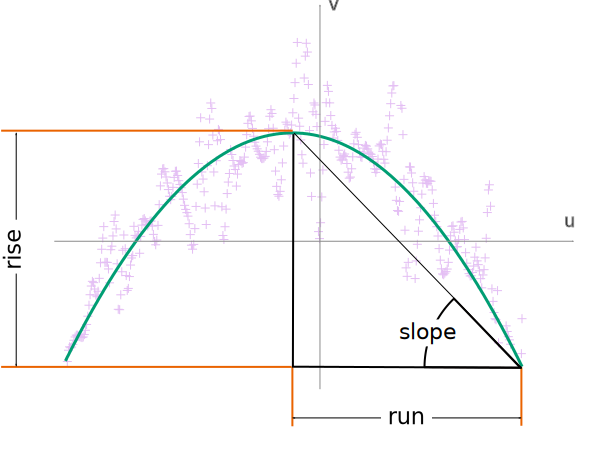
\includegraphics[width=0.8\textwidth]{figures/line_deviation}
\caption{How edge curvature is measured. Keep in mind that the edge modeled
here with the parabola would look pretty straight in the actual image --- it
just looks so curved here because of the high magnification of the v-axis
(\emph{rise} is only 0.06 pixels).}
\label{fig:line_deviation}
\end{figure}

The only reliable, safe way to compare the output of MTF Mapper between
different images captured using the same camera (say, an f/2.8 vs an f/4
image capture) is to use the pixel coordinates (\emph{edge\_x},
\emph{edge\_y}) of a 
measurement from image A to find the closest corresponding measurement from
image B, assuming you do not move around the camera too much, or rotate the
chart or something like that (in which case you can use the Monkres
assignment algorithm to calculate the correct pairing). Please do not rely
on the order of the rows of the \texttt{edge\_mtf\_values.txt} and
\texttt{edge\_sfr\_values.txt} files.

\newpage

\section{Autofocus fine-tuning}
\label{sec:autofocus}

\subsection{The method}
%
\begin{figure}[bp!]
\centering
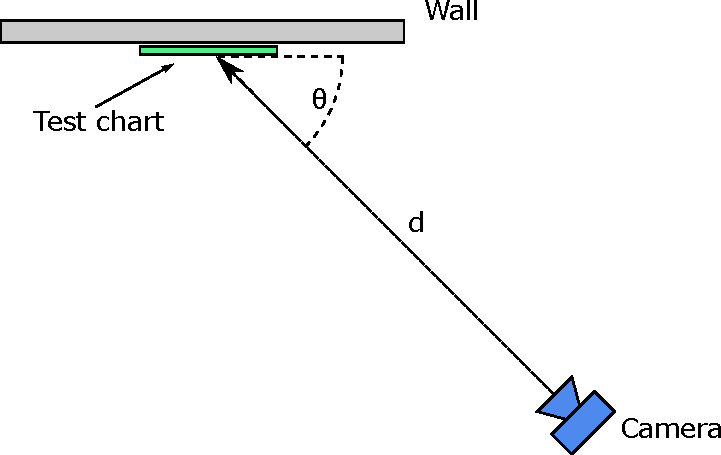
\includegraphics[width=0.65\textwidth]{figures/af_setup}
\caption{Illustration showing the top view of the autofocus calibration
set-up}
\label{fig:af_setup}
\end{figure}
%
\begin{figure}[bp!]
\centering
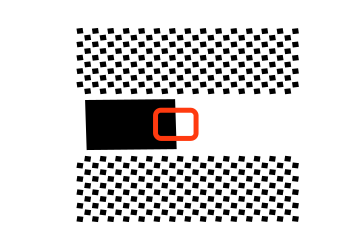
\includegraphics[width=0.65\textwidth]{figures/af_sensor_placement}
\caption{Where to place your autofocus sensor}
\label{fig:af_sensor_placement}
\end{figure}
%
The following steps can be used to calibrate the autofocus fine-tuning of a
DSLR:
\begin{enumerate}
    \item Figure~\ref{fig:af_setup} illustrates the basic set-up. The
distance $d$ is the ``distance to chart'', and the angle $\theta$ is the
``angle with respect to the test chart''.
    \item Print out the test chart at a large enough scale. Ideally, your
test chart must be large enough so that you can use it at a distance of
$30\times$ the focal length of your lens. Appendix~\ref{sec:tips} offers
some advice on printing your test charts.

Position your camera so that you see the chart from an angle of at least $45^\circ$ --- the idea is that you
want some of the small blocks to be in front of the plane of focus, and some
of the blocks behind the plane of focus; this is easier to achieve at angles
of $45^\circ$ and smaller. The reference edge (Section~\ref{sec:profile_mode}) should be
exactly at the plane of focus, but since you are reading this, I take it you
are still trying to adjust the autofocus fine-tuning to achieve this.

  \item You must use a tripod, and it is recommended that you use a remote
shutter release or a timed shutter release to minimise vibrations.

   \item You should have enough
light for an exposure value of 10--11 (for example, ISO 100 F/1.8 at 1/320
s), which translates into about 2500--5000 lux. This amount of light is 
required to achieve consistent performance from
the AF sensor. I use indirect sunlight to reach these levels.

    \item Set your camera to AF-S (single-servo AF). Select a single AF
point --- the centre AF sensor is recommended. This is critical, as any
other AF mode / sensor selection will not produce the desired results.
On Nikon bodies, I like
to use the AF-ON mode so that the camera only focuses when I ask it to. For
adjusting your AF fine tuning settings, you should use a single AF
operation, i.e., press and hold the AF-ON button until focus lock is
achieved, then release the button. Do not focus a second time.

    \item Aim the AF sensor reticule so that it straddles the reference edge
(see Figure~\ref{fig:af_sensor_placement}). Take care that the autofocus sensor
is sufficiently far away from other edges (e.g., the horizontal edges of the
reference block in Figure~\ref{fig:af_sensor_placement}, or any of the small
blocks). Keep in mind that the actual sensing area of the autofocus sensor
is typically larger than the reticule you see in the viewfinder, so leave
some padding.

    \item Manually set the focus of your lens to the near limit, or to
infinity.

    \item Initiate one AF operation.
   
    \item Capture a shot of the test chart. Lower ISO values are better, since MTF
measurements are more variable if you have a lot of noise.

    \item Feed the captured image through MTF mapper to produce a profile
(such as illustrated in Figure~\ref{fig:sample_profile}. The vertical blue
line denotes the position of the autofocus reference edge (at least, the one
you should have been using to focus \ldots). The green curve (or red
points) records the MTF50 values measured along the long axis of the image.
Since the test chart was at a $45^\circ$ angle with respect to the lens
axis, the long axis of the image is a measure of the distance from the
camera. MTF50 values measured at different $x$-values (in the
Figure~\ref{fig:sample_profile}) thus indicate the
sharpness, or degree of focus, at that specific distance from the camera.
The peak of the green curve represents the plane of focus --- the objective
is to line up the peak of the green curve with the blue vertical line.

    \item This procedure (steps 7--10) should now be repeated at various autofocus
fine-tuning settings on your camera. You should be able to see the peak of
the green curve shift left or right as you adjust this value. I recommend
capturing your images in batches, first stepping your autofocus fine-tuning
through the range in large steps, running the images through MTF mapper, and
then repeating this in the optimal range with smaller steps until you are
satisfied that you have calibrated your autofocus fine-tuning to the desired
level of accuracy.
\end{enumerate}

\subsection{Caveats and disclaimers}
Please note that this procedure of calibrating autofocus fine-tuning on your
DSLR is based on some of my own assumptions, which have not been tested
rigorously before the release of this software. Here follows some
background; you are most welcome to skip this section.

Phase-detection autofocus in DSLR cameras works by collecting light from
opposite sides of the lens (the aperture, really), if the article on
Wikipedia is
accurate\footnote{\url{http://en.wikipedia.org/wiki/Autofocus}}. These two
beams of light are steered to two independent linear sensors --- I suspect
that they are simply small strip-like CMOS sensors nowadays. Using
cross-correlation, the AF module then measures the phase shift between the
data collected from the two linear sensors; this phase shift will directly
correspond to the degree of defocus. With this information, the AF module
can then drive the AF motor by approximately the correct amount to
eliminate the phase difference between the signal received by the two
linear sensors, which should bring the object under the relevant AF sensor
into focus.

So the real question is: what algorithms do the AF modules really use to
measure the phase shift? Well, I currently do not know. If you design AF
modules, please fill me in, and I can update my test charts to agree more
closely with what the AF modules expect to see. Many AF test charts  are
available on the Internet, however, most of them use thick line (bar-shaped)
target to draw the AF sensor's attention. Someone on the Internet (now,
there is a reference you can count on) pointed out that bar targets are a
poor choice, because they may be too thin for the AF sensor to detect. I
found this argument appealing, because the AF sensor must have limited
resolution. There is an additional problem with a bar target: which edge of
the bar target is the AF module going to focus on? And this process led me
to the design of my own test charts. Rather than using a bar as an AF
target, why not use a step edge? If the AF module really does use
cross-correlation to measure the phase difference, then a step edge would
produce the best possible results. There would also be no ambiguity as to
where the sensor is focusing, since the step edge only has one feature to
focus on.

Well, it seems to work. At least for my camera bodies and lenses.

I also found it annoying to have to use visual inspection to determine
whether I have set the autofocus fine-tuning optimally. Visual
inspection certainly is a quick way to evaluate the results in the field, but I want to see some
objective data. I want to \emph{know} that I have calibrated my lenses
perfectly. Anyhow, if you have made it this far, you probably understand.
MTF50 is certainly not the final word on image acuity (read the excellent
Zeiss papers for a start), but it does provide a reasonable relative measure
for the autofocus calibration problem. The MTF50 estimates extracted by MTF
Mapper are reasonably accurate (see Appendix~\ref{sec:accuracy}), at least as
far as internal consistency goes with my own edge image generator. You should 
be able to obtain repeatable results within a 5\% relative margin.

Lastly, you should know one very important thing about autofocus systems:
they are not perfect. The tolerances of the AF system (AF module, lens
drive accuracy, etc.) are such that they strike a balance between speed and
accuracy. 

With MTF mapper, you can empirically observe this effect:
manually set focus to infinity, switch to AF, capture image. Now select near
focus (manually), switch to AF, capture image. Comparing the profile plots
of produce by MTF mapper you should be able to see which image was captured
from which direction, and the distance between the peaks in the profiles
should roughly correspond to this ``zone of acceptable focus'' for that
subject distance and magnification.

\section{Cropped images, or single region-of-interest images}
\label{sec:single_roi_mode}
Occasionally it is not possible to use an MTF Mapper test chart. This could
be because a review site only uses an older ISO 12233:2000 test chart, or
because you are using a back-lit razor blade (the ultimate DIY reference edge if
you do not have an optics lab). Unfortunately MTF Mapper cannot
automatically isolate the edge of interest in such images, however, 
it is still possible to use MTF Mapper to analyze cropped regions of such
images.

Figure~\ref{fig:single_roi_mode} shows one example of such a cropped image
of a slanted edge. To use such an image with MTF Mapper, just pass the
\texttt{--single-roi} option to the command-line tool, or open your files
using the \textsf{File/Open single edge images(s)} GUI option. Of course, the only
sensible visual output for such an input image would be the \textsf{Annotated
image} option; from there you can view the SFR curve in the gui. (Or see the
\texttt{-q} output option for the command-line tool).

\begin{figure}[!ht]
\centering
\begin{subfigure}[c]{0.15\textwidth}
    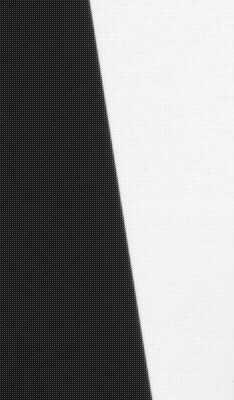
\includegraphics[width=\textwidth]{figures/single_roi_input}
    \caption{Input image}
\end{subfigure}
\qquad
\begin{subfigure}[c]{0.15\textwidth}
    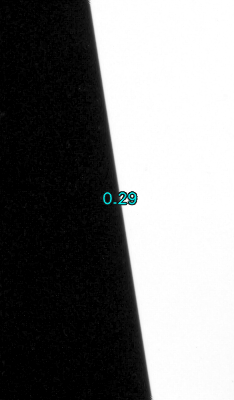
\includegraphics[width=\textwidth]{figures/single_roi_output}
    \caption{Annotated image}
\end{subfigure}
\quad
\begin{subfigure}[c]{0.6\textwidth}
    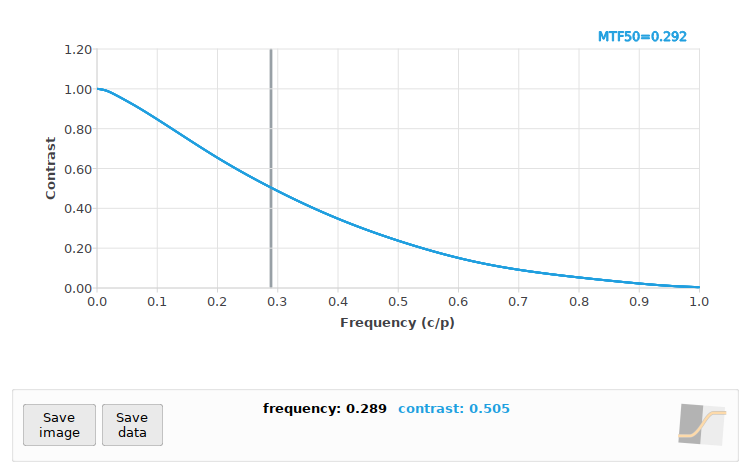
\includegraphics[width=\textwidth]{figures/roi_sfr_example}
    \caption{SFR curve}
\end{subfigure}
\caption{Single ROI example}
\label{fig:single_roi_mode}
\end{figure}

The edge can be in either a vertical or horizontal orientation, and it does
not matter on which side of the image the dark side of the edge
appears.

\section{Lens distortion correction}
\label{sec:lens_distortion}
Lens distortion can have a fairly significant impact on slanted-edge MTF
measurements. If a slanted edge in the captured image is no longer straight,
but rather curved, the measured MTF will decrease. The magnitude of the
impact of lens distortion on MTF measurements is highly dependent on the
length of the edge relative to the magnitude of the distortion. If the edge
is short enough, or the distortion is weak enough, then you can get away
without explicitly correcting for distortion. For the other cases, there 
are several strategies to deal with lens distortion:
\begin{description}
\item[Undistortion using an ideal lens model:]

Use a pre-defined lens model to ``straighten'' the edges before applying the
slanted edge method. This option is appealing if you are dealing with a
fisheye lens, and you wanted to undistort the image anyway. A modified
version of the slanted-edge method is required to make this work; you cannot
simply undistort the image before passing it to MTF Mapper, since this will
produce unrealistically low measurements in areas with large compression,
such as the corners of a fisheye lens.

MTF Mapper offers support for this type of lens distortion correction
through the `Equiangular' and `Stereographic' options under the Lens
distortion correction panel of the \textsf{Preferences} dialog. For both
these models it is compulsory to specify the focal length of the lens in the
field provided. In addition, the `Pixel size' field in the Advanced panel
must also be set to the correct value (sensor photosite pitch, in micron),
and the `Line pairs/mm units' option must be enabled in the Flags panel.

Lastly, keep in mind that the two supported lens models do not allow for any
additional deviation from the ideal equiangular or stereographic fisheye
lenses.

\item[Undistortion using a fitted model:]

Fit a parametric lens distortion model to ``straigthen'' the edges, using
the image of the test chart itself to estimate the distortion parameters.
Think of it as an automatic lens undistortion model; once these model
parameters have been estimated the internal implementation is basically the
same as for the fisheye undistortion models. In my limited testing, this
automatic lens undistortion feature worked just fine when applied to fisheye
lens images, although I did not test circular fisheye lenses.

MTF Mapper supports this approach through the `radial' option under the Lens
distortion correction panel of the \textsf{Preferences} dialog. There is no
requirement to specify a pixel size, or focal length, or to enable the `Line
pairs/mm units' option.

The main disadvantage of this approach is that it is inherently a two-pass
scheme, thus it will be noticebly slower than other undistortion options.

\item[Direct modeling of curved edges:]

Treat each edge in the image independently as a curve, rather than a
straight line. This requires a modified implementation of the slanted-edge
algorithm, but other than requiring a model-fitting step to approximate each edge,
relatively little extra work has to be performed, making this approach
almost transparent in terms of cost. This method has the distinct advantage
of not requiring a lens model, and not requiring an undistorted image to be
produced. The usual approach is to fit a quadratic polynomial (i.e., a
parabola) through the curved edge; this is a pretty good approximation for
most types of lens distortion, excluding `moustache' distortion. If you have
to deal with `moustache' distortion a piecewise-quadratic polynomial fits
much better.

MTF Mapper now uses the piecewise-quadratic curved edge approach to dealing
with lens distortion by default. You can try the garden-variety quadratic
curved edge model by selecting the `quadratic' option under the Lens
distortion correction panel of the \textsf{Preferences} dialog. If you want
to revert to a plain-vanilla straight edge model, choose the `none' option.

\end{description}

\section{Frequently Asked Questions}
\begin{enumerate}
  \item Your program gave me a value of $x$ cycles per pixel. Is this any
good? \emph{Answer}: According to Norman Koren
(\url{http://www.imatest.com/guides/modules/sfr}), a value of 0.33 cycles
per pixel is pretty good \emph{for unsharpened raw images} (emphasis mine).
This is somewhat misleading, though, since expressing MTF50 as c/p is not
independent of the sensor resolution, and Norman may have been referring to
an 8 MP sensor. Take, for example, a sample of the
Nikkor 35 mm f/1.8 prime lens on a D40 body. This combination achieves MTF50
values of around 0.28 c/p. The same lens on a D7000 body achieves around
0.22 c/p. If these values are expressed as line pairs per millimetre
(lp/mm), we actually see 36 lp/mm on the D40, and 46 lp/mm on the D7000. In
this case, it means that the lens is actually able to resolve more detail
than what the D40 could capture. This also explains why I suddenly thought
the lens looked softer on the D7000 --- the per-pixel sharpness was
definitely lower, even though the effective sharpness was higher.

So while c/p units are convenient because they do not require knowledge of the
pixel (or sensor) size, they are not portable to other sensors for the very
same reason. 
I prefer to use lp/mm when comparing lenses, but c/p are more natural for
synthetic images. 
  \item Cycles per pixel? I wanted lw/ph or lp/mm! \emph{Answer}: Support
has been added for lp/mm by specifying a pixel size with the
\verb+--pixelsize+ option.
You can also convert manually using the
following relationship:
    \begin{eqnarray}
	\mathrm{MTF50}_{\mathrm{lp/mm}} = 
	  \frac{\mathrm{MTF50}_{\mathrm{c/p}} \times h_{\mathrm{pixels}}}{h_{\mathrm{mm}}} \\
        \mathrm{MTF50}_{\mathrm{lw/ph}} = 2 \times \mathrm{MTF50}_{\mathrm{c/p}} \times h_{\mathrm{pixels}} 
    \end{eqnarray}
where $h_{\mathrm{mm}}$ is the image height in mm, and $h_{\mathrm{pixels}}$
is the image height in pixels.
\end{enumerate}

\section{Acknowledgements}
Although I am the sole author of MTF Mapper, quite a few of the ideas that
have gone into MTF Mapper were contributed by users, or their request for
features motivated me to implement said functionality. I extend thanks to the following
entities:
\begin{itemize}
\item Jack Hogan
\item Ed Dozier
\item craig66 (of DP Review forums)
\item Jim Kasson
\item Bernard Delley
\item Alpa, who funded the development of the \textsf{Focus position}
functionality
\item Brandon Dube
\end{itemize}

\appendix

\section{Tips for printing the test charts}
\label{sec:tips}
I have printed the MTF Mapper test charts using a variety of printers, and
have the following advice to offer:
\begin{itemize}
  \item If you are printing on paper, you should aim to use the thickest
  paper available. Something like 120 g/m$^2$ is probably the bare minimum.
  All my charts printed on standard 80 g/m$^2$ paper warped horrendously
  with changes in humidity.
  \item The test charts work best when they are quite flat. I have worked
  with an A0 print of the perspective chart that was simply taped to a
  plastered wall, and everything seemed to be fine. If, on the other hand,
  you are using the grid chart to look for MTF variations in the focal plane, 
  then it is critical to keep the chart perfectly
  flat. I have found that foam board works very well, especially if you use
  a spray glue to fix the printed chart to the foam board.
  \item Even spray glue combined with a foam board is not good enough to
  prevent thin paper from warping due to changes in humidity. If you plan on
  using a chart more than once, you \emph{must} use thick paper. It might
  also help if you use mechanical clamps (e.g., Bulldog clips) in stead of
  spray glue to fasten your chart to the backing.
  \item I have yet to try this myself, but a local printer can print on a
  self-adhesive vinyl sheet. This should be immune to humidity, but
  obviously this will be much more expensive than printing on plain paper.
  \item Another untested idea is to use a laser-marking (laser-engraving)
  machine to ``print'' onto a painted aluminium sheet. Let me know if 
  you've tried this!
  \item Print quality is probably not critical when using the perspective
  charts --- I have used badly printed (streaky, not quite solid) charts,
  and that seemed to be OK on an A0 scale.
  \item Print the largest chart you possibly can for a given focal length.
  In practice, I have found that the A0-size charts work very well for
  lenses shorter than 50 mm, since they allow me to keep the chart at a 
  realistic distance. I have yet to perform extensive tests on A4 charts, 
  but I suspect they are only safe to  use with longer focal lengths 
  (e.g., 200 mm or longer). Furthermore, at greater distances, you can get
  away with lower quality prints --- 300 DPI prints are fine on an A0 chart,
  but may become a problem on A4 charts.
  \item Test chart quality is critical if you want to obtain \emph{absolute}
  results, such as when you want to compare your results to other sources
  (online, etc.). If you are just evaluating the relative performance of two
  lenses, e.g., two copies of the same lens, or two different brands of 50
  mm prime lenses, then you can get away with a lower quality test chart.
\end{itemize}

\newpage

\section{Accuracy assessment}
\label{sec:accuracy}
The evaluation of the accuracy of an implementation of the slanted-edge
method can become rather complicated. The MTF Mapper blog
(\url{https://mtfmapper.blogspot.com}) contains quite a few articles on this
topic. For now, I will just include one graph illustrating the accuracy of
MTF Mapper compared to two other popular implementations: Imatest and
Quick MTF. The test involves generating a large number of test images
containing slanted edges, repeating the rendering of each image with a
different simulated (expected) MTF50 value, in the presence of a low (but
realistic) level of image noise. Afterwards, the three contenders were used
to measure the MTF50 value of the simulated edges. I choose to use the
\emph{relative} error, meaning that the error is expressed as
\begin{displaymath}
\mathrm{err}_\mathrm{relative} = 
100\cdot\frac{\mathrm{MTF50}_\mathrm{measured} -\mathrm{MTF50}_\mathrm{expected}}{\mathrm{MTF50}_\mathrm{expected}}
\end{displaymath}
since this makes the range of errors comparable across different expected
MTF50 values (or otherwise the blurry edges appear to have almost no error
relative to sharp edges).

\begin{figure}[ht!]
\centering
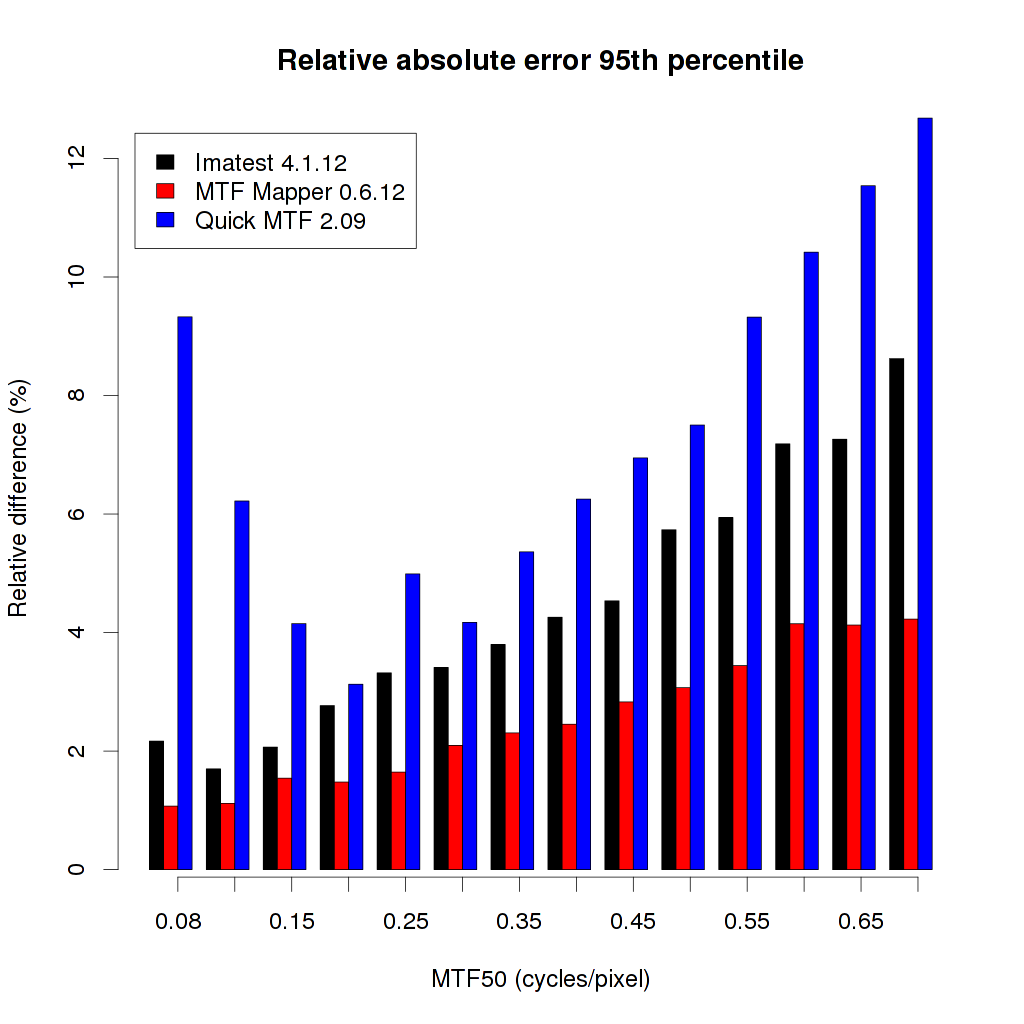
\includegraphics[width=0.8\textwidth]{figures/p95_comparison}
\caption{Accuracy comparison: MTF Mapper vs. Imatest vs. Quick MTF}
\label{fig:se_comparison}
\end{figure}

At any rate, over the multiple samples at each simulated MTF50 value, the
$95^\mathrm{th}$ percentile of $|\mathrm{err}_\mathrm{relative}|$ was
computed; the results are presented graphically in
Figure~\ref{fig:se_comparison}. To interpret this graph: 95\% of the 240
edges with an expected MTF50 of 0.25 cycles/pixel were measured with MTF
Mapper to have an estimated MTF50 value between about 0.245 and 0.255, i.e.,
the measurements were within 2\% (roughly the height of the red bar at 0.25
cycles/pixel on the x-axis).

Under these conditions MTF Mapper is
\emph{at least} as accurate as Imatest 4.1.12, and definitely more accurate
than Quick MTF. Informal experiments with the slanted-edge plugin for ImageJ
as well as Mitre SFR indicate that those implementations are significantly less
accurate than MTF Mapper.

\section{User manuals for individual applications}
\label{sec:manpages}
\begin{center}
(Rest of this page left blank intentionally)
\end{center}
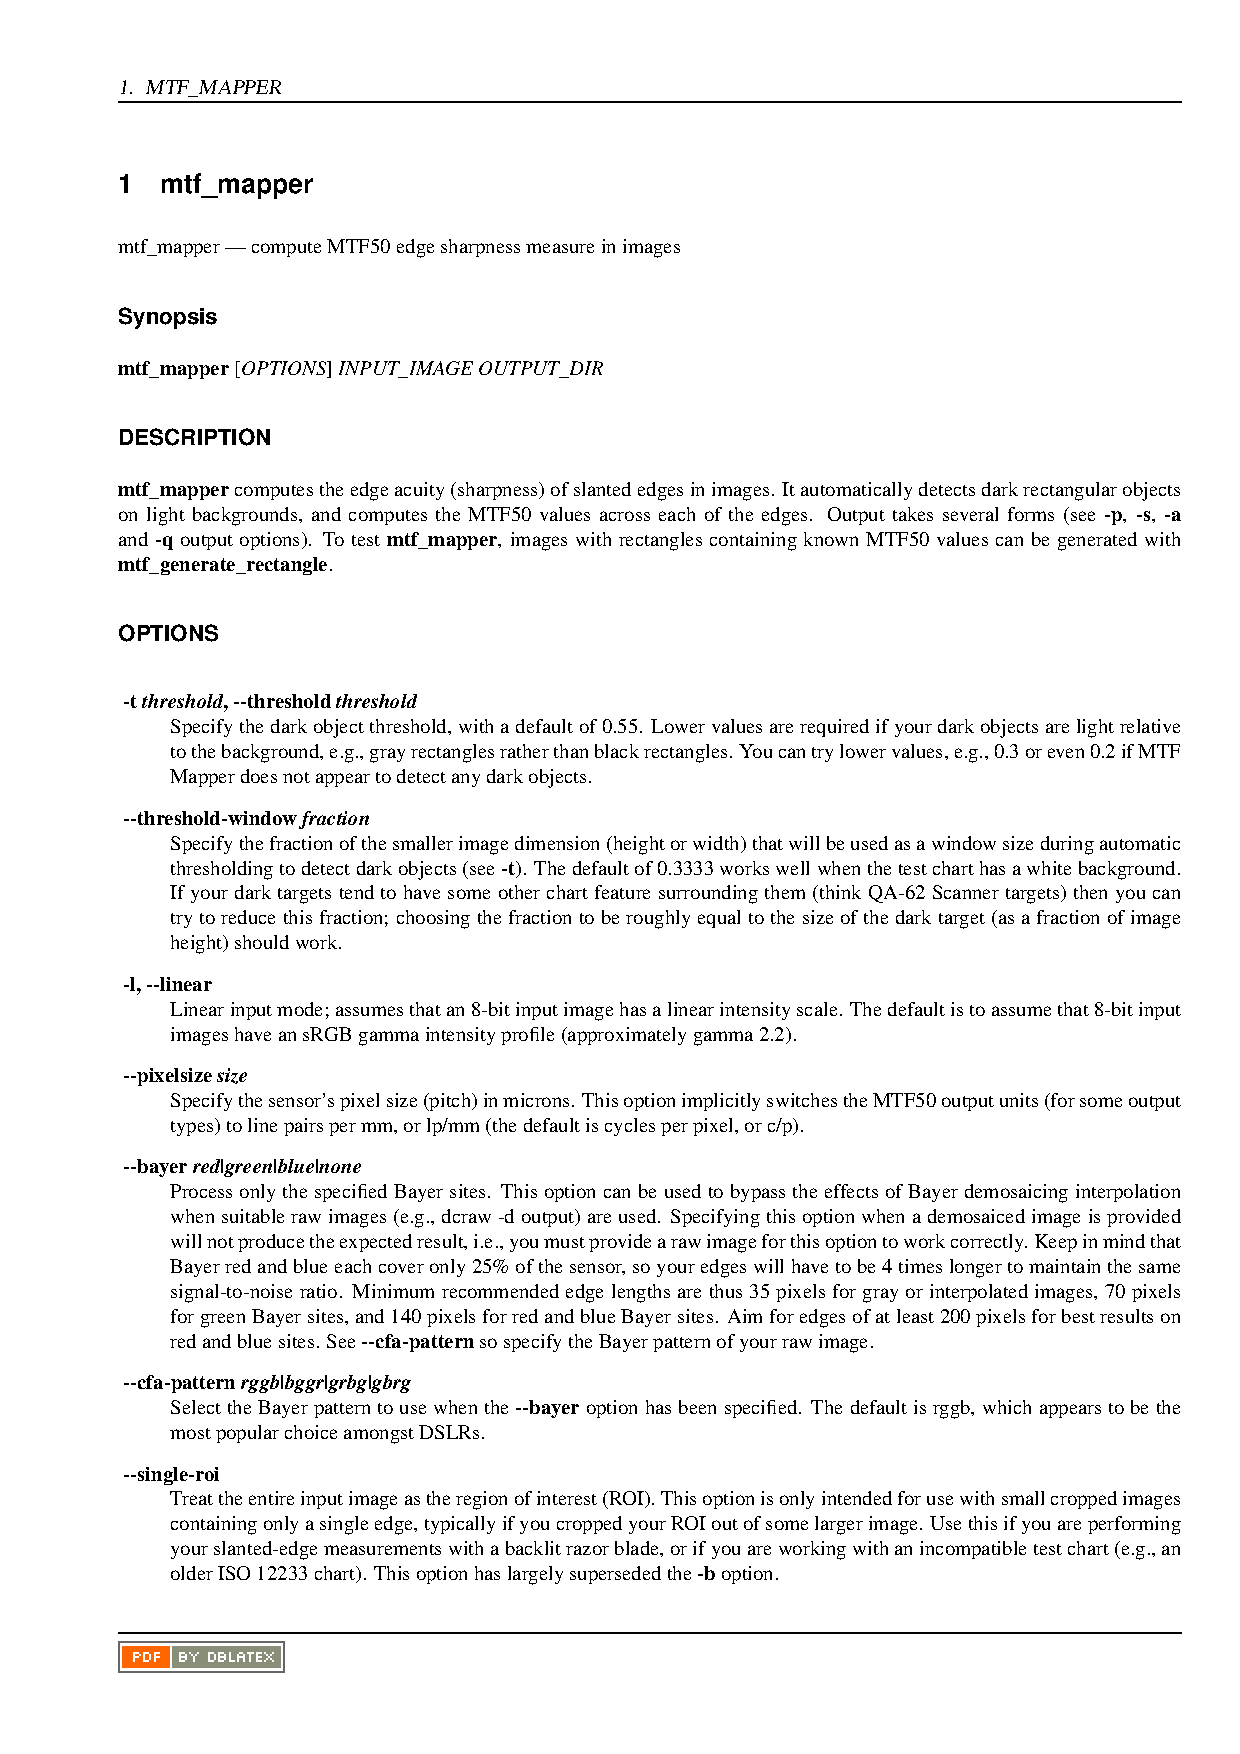
\includepdf[pages={1-5}]{figures/mtf_mapper_man.pdf}
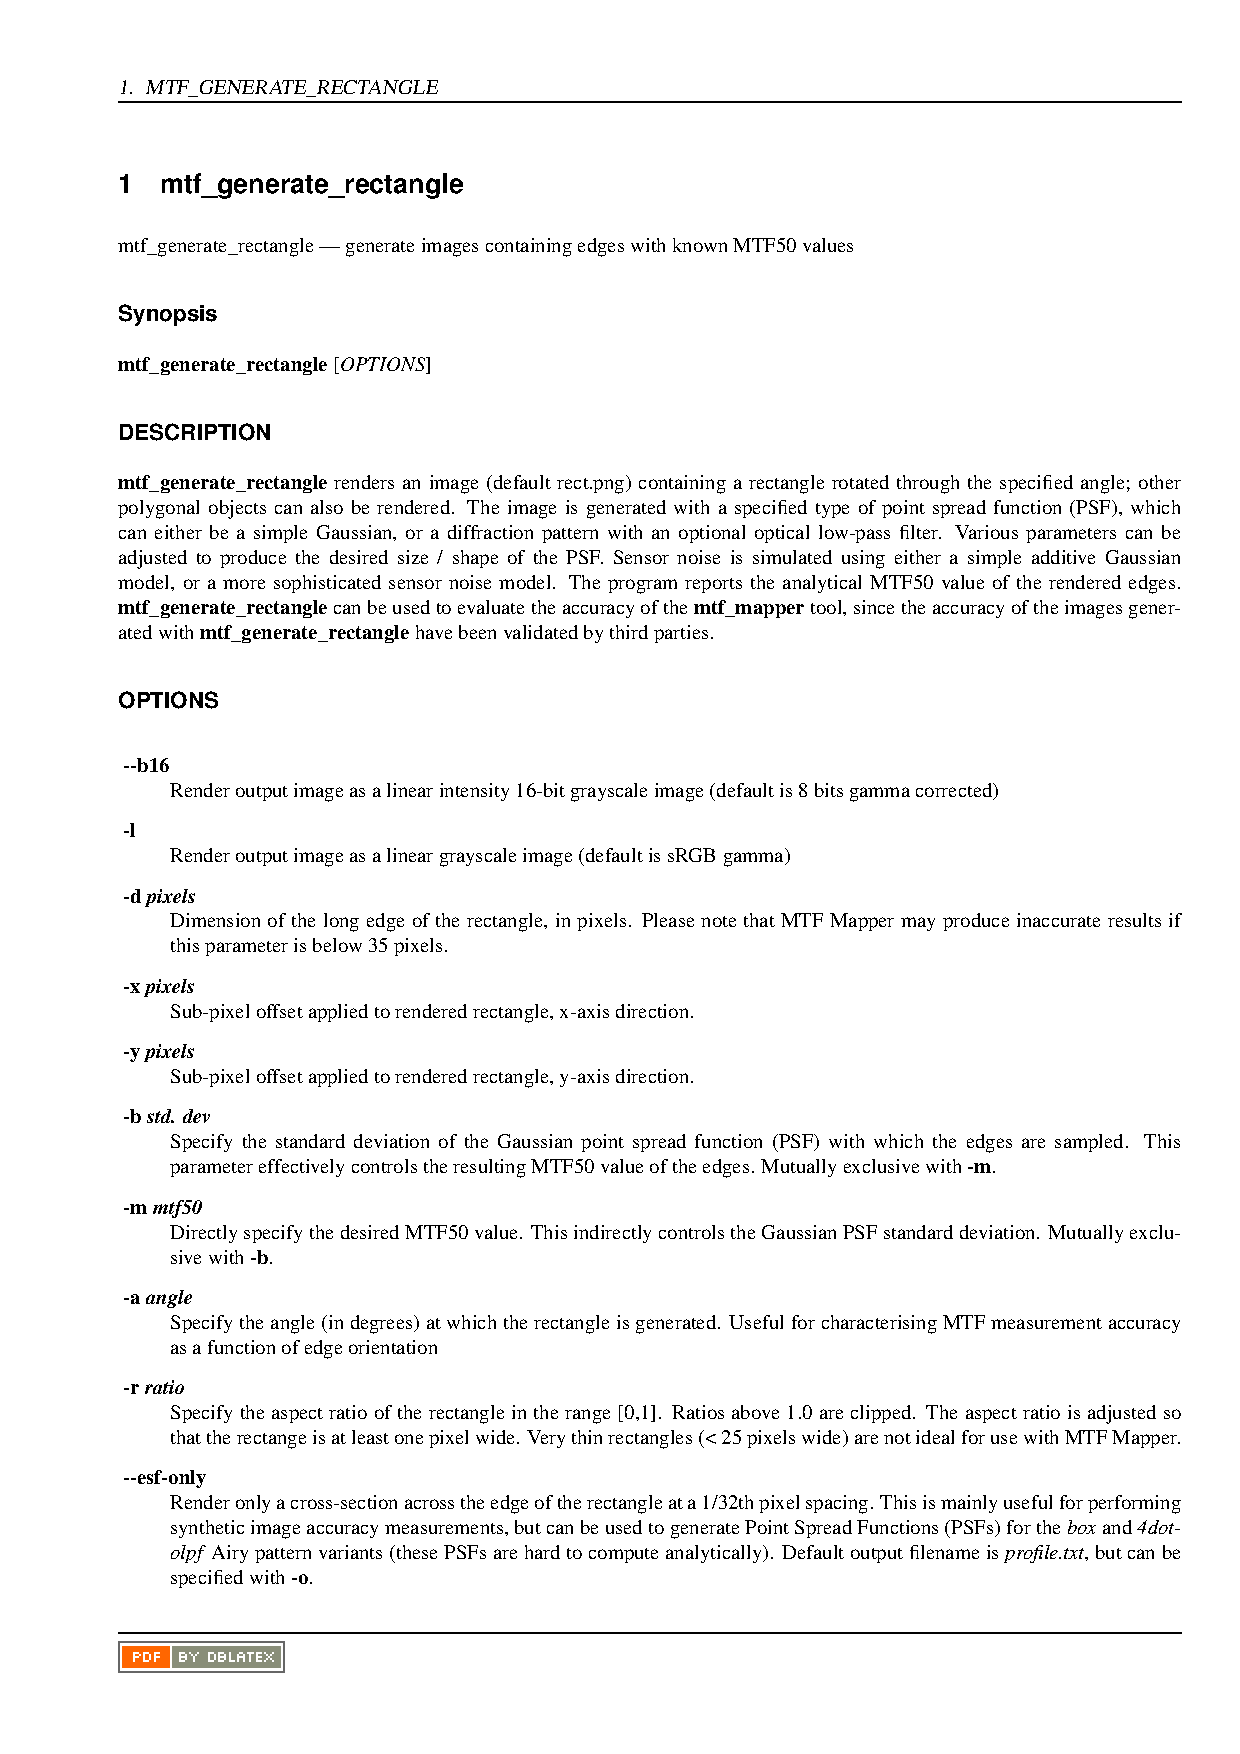
\includepdf[pages={1-4}]{figures/mtf_generate_rectangle_man.pdf}
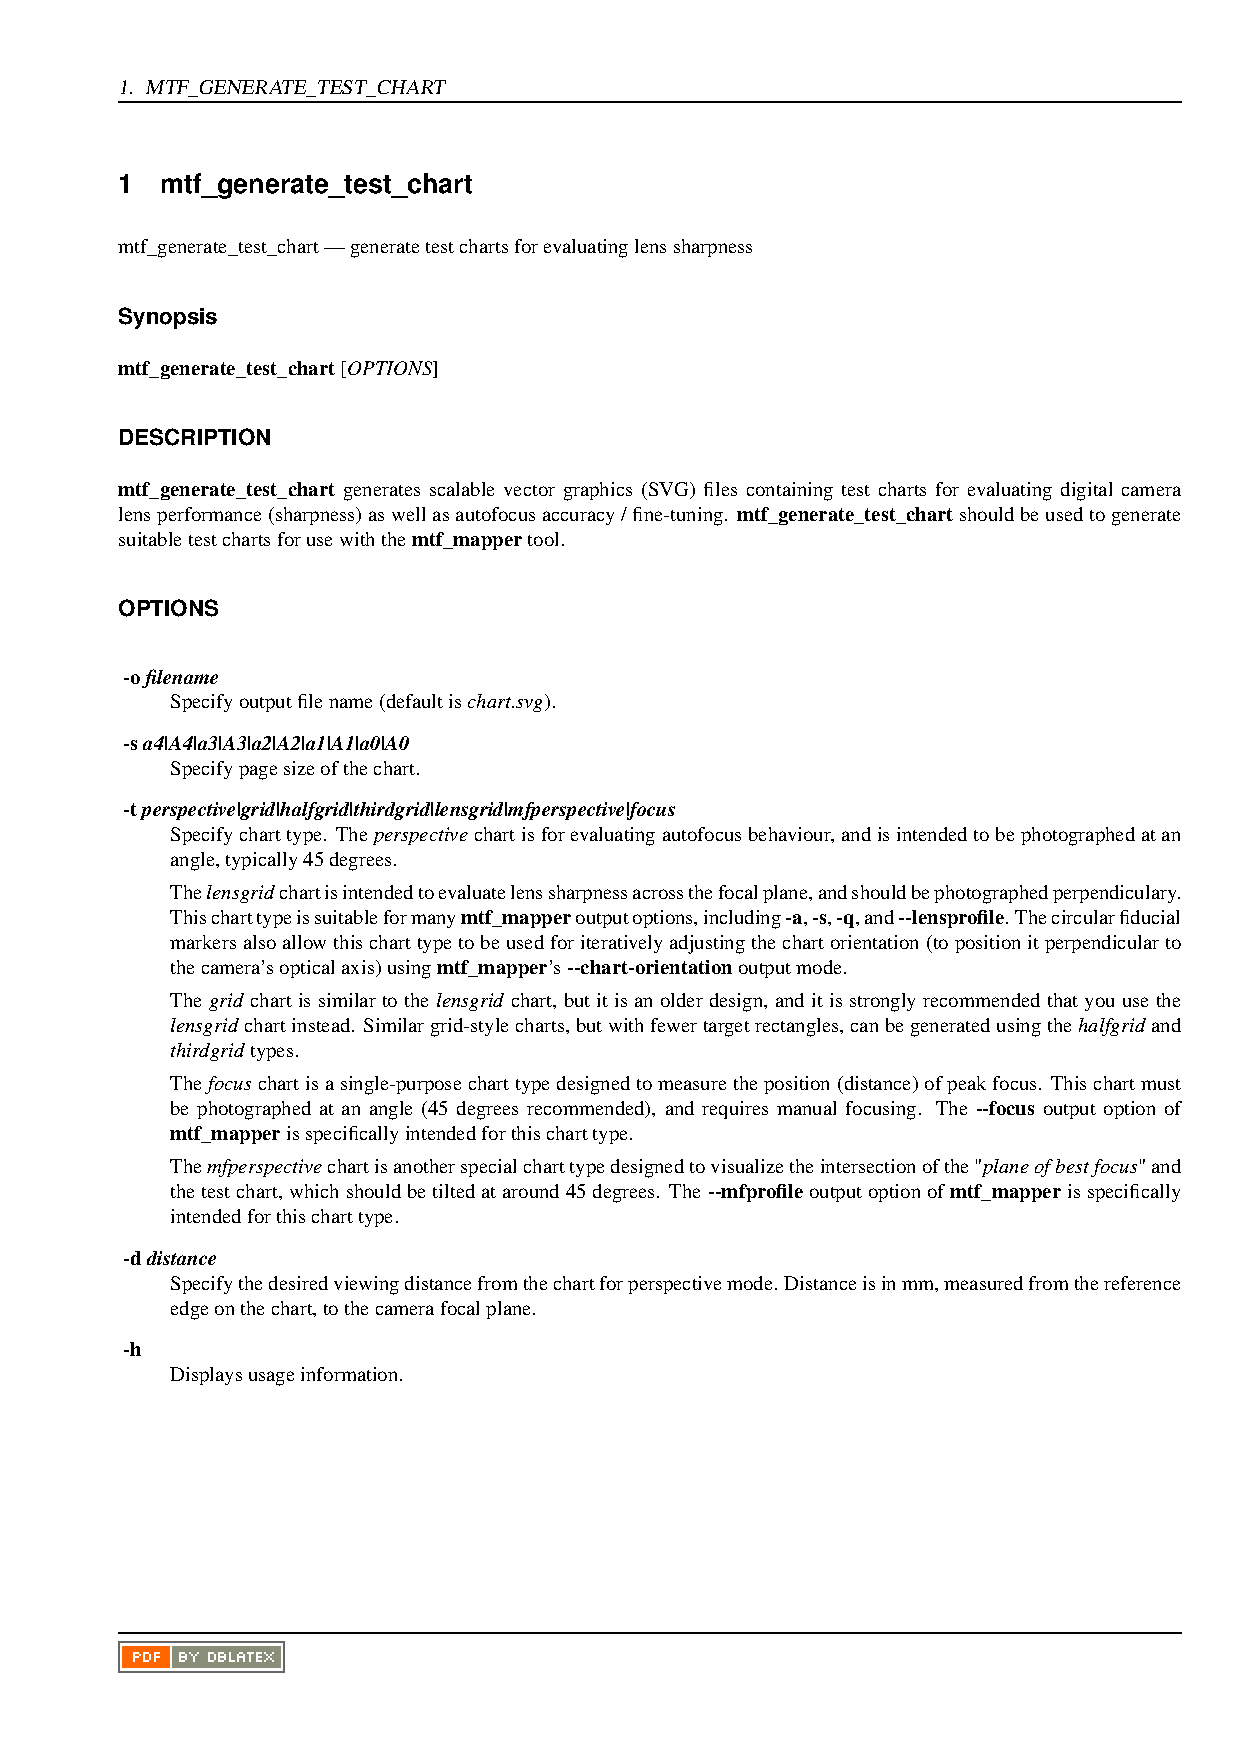
\includepdf[pages={1}]{figures/mtf_generate_test_chart_man.pdf}


\begin{thebibliography}{9}
\bibitem{khom} Kohm, K., \newblock{Modulation transfer function measurement
method and results for the Orbview-3 high resolution imaging
satellite}, \newblock{Congress International Society for Photogrammetry and Remote
Sensing}, 20:12--23, 2004.
\bibitem{bradley} Bradley, D. and Roth, G.,
\newblock{Adaptive thresholding using the integral image},
\newblock{\textit{Journal of Graphics, GPU, \& Game Tools}}, \textbf{12(2)}:13--21,
2007.
\bibitem{chang} Chang, F., Chen, C.J., Lu, C.J.,
\newblock{A linear-time component-labeling algorithm using contour tracing
technique},
\newblock{\textit{Computer Vision and Image Understanding}}, \textbf{93(2)}:206--220,
2004
\end{thebibliography}

\end{document}
